%% (C) 2009 Stefan Heule
%% 
%% Licence: Creative Commons Attribution-Share Alike 3.0 Unported
%% http://creativecommons.org/licenses/by-sa/3.0/
%% 
%% Einen Teil der Inhalte wurde (angepasst) von der Zusammenfassung von
%% Thorben Bochenek, Licia Huber, Pascal Spörri, Patrick Tremp, Mathieu Jean-Daniel
%% übernommen.
%% 

\documentclass[portrait,a4paper,titlepage]{article}

\usepackage[utf8x]{inputenc}
\usepackage{german}
\newcommand\tab[1][1cm]{\hspace*{#1}}

\usepackage{amssymb, amsfonts}
\usepackage{amsmath}
\usepackage[e]{esvect}

\usepackage{graphicx}
\usepackage{pdfpages}

\usepackage{xcolor}

\usepackage{listings}
\lstset{
	basicstyle=\ttfamily\mdseries,
	identifierstyle=,
% 	stringstyle=\color{green},
	numbers=none,
	inputencoding=utf8x,
	keywordstyle=[1]\bfseries\color{blue},
	keywordstyle=[2]\bfseries\color{teal},
	keywordstyle=[3]\bfseries\color{red},
	keywordstyle=[4]\bfseries\color{yellow},
%	numberstyle=\tiny,
%	stepnumber=10,
	breaklines=true,
	frame=none,
	showstringspaces=false,
	tabsize=4,
	commentstyle=\color{gray},	
	captionpos=b,
	float=htbp,
}

\usepackage{geometry}
\geometry{a4paper, left=10mm, right=10mm, top=20mm, bottom=20mm} 

\usepackage{multicol}  
\columnsep24pt
\columnseprule0.1pt

% uply greek letters :)
\renewcommand{\phi}{\varphi}
\renewcommand{\epsilon}{\varepsilon}

% aufzählungszeichen
%\renewcommand{\labelitemi}{-}
\renewcommand{\theenumi}{\roman{enumi}}
% d in integralen, etc. (z.b. integral f(x) *d*x)
\newcommand{\rmd}{\mathrm{d}}
% fette mathematische symbole
\newcommand{\bs}{\boldsymbol}
% mathcal
\newcommand{\mc}{\mathcal}
% norm
\newcommand{\norm}[1]{| \!\:\! | #1 | \!\:\! |}

% formeln innerhalb von text -> normale formelndarstellung
\newcommand{\ds}{\displaystyle}

% pfeil
\newcommand{\arr}{\rightarrow}

% integral mit grenzen oben und unten
\newcommand{\intl}{\int\limits}

% zahlenmengen
\newcommand{\R}{\mathbb{R}}
\newcommand{\Z}{\mathbb{Z}}
\newcommand{\N}{\mathbb{N}}
\newcommand{\C}{\mathbb{C}}

% todo
\newcommand{\todo}[1]{$\ggg$ \textbf{TODO} [#1]}

% shorter then \begin{comment}..\end{comment}
\newcommand{\nop}[1]{}

% hyperref / svn
\usepackage[colorlinks=false,pdfborder = {0 0 0 0}]{hyperref}
\usepackage{svn-multi}
\svnid{$Id: main.tex 26 2009-08-09 18:56:51Z stheule $}

% paragraphe nummerieren und titel auf eigener zeile
\setcounter{secnumdepth}{4}


\begin{document}

\author{Stefan Heule}
\title{Digitaltechnik Zusammenfassung 2009
\thanks{Licence: Creative Commons Attribution-Share Alike 3.0 Unported (\url{http://creativecommons.org/licenses/by-sa/3.0/})}
{\\ \small Revision \svnrev}
}
\date{\today}
\maketitle



% alle Kapitel werden aus einzelnen Dateien eingebunden
\section{Kombinatorische Schaltungen}
A combinational circuit outputs, only depend on it's inputs therefore it is memoryless, a sequential circuit output's depend both on it's current and old inputs, it has memory. A combinational circuit has the following properties:
\begin{enumerate}
	\item Every circuit element is combinational.
	\item Every node of the circuit is either designated as an input to the circuit or connects to exactly one output terminal of a circuit element.
	\item The circuit contains no cyclic paths: every path through the circuit visits each circuit node at most once.
\end{enumerate}
	
	\begin{multicols}{2}
	\subsection{Gatter}
		\renewcommand{\arraystretch}{1.5}
		\begin{tabular}{r  || c c c c}
			               &   Logik      &   Algebra                 &   Schaltbild  & Verilog   \\ \hline\hline
		OR		        &   $x \lor y$          &   $x + y$                 
										&   
\includegraphics[height = 11pt]{images/gatter/or}    &     \verb+x || y+       \\
		NOR	    &   $\lnot(x \lor y)$    &   $\overline{x + y}$      
										&   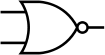
\includegraphics[height = 11pt]{images/gatter/nor}    &                       \\\hline
		AND	         &   $x \land y$        &   $x \cdot y$             
										&   
\includegraphics[height = 11pt]{images/gatter/and}    &     \verb+x && y+         \\
		NAND	    &   $\lnot(x \land y)$  &   $\overline{x \cdot y}$  
										&   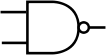
\includegraphics[height = 11pt]{images/gatter/nand}    &                     \\\hline
		NOT	          &   $\lnot x$            &   $\overline{x}$          
										&   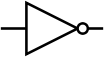
\includegraphics[height = 11pt]{images/gatter/not}    &     \verb+!x+         \\\hline
		XOR	    &   $x \ne y$           &   $x \oplus y$            
										&   
\includegraphics[height = 11pt]{images/gatter/xor}    &     \verb+x ^ y+             \\\hline
		XNOR	        &   $x = y$             &   $\overline{x \oplus y}$ 
										&   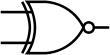
\includegraphics[height = 11pt]{images/gatter/xnor}    &     \verb+x == y+       \\\hline
			       &   $x \to y$           &   $x \le y$        
										&   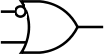
\includegraphics[height = 11pt]{images/gatter/implies}    &   \verb+!x || y+       \\
		\end{tabular}
	
	\subsection{Wahrheitstabellen}
	A literal can have the value of 1, 0, x if it is a illegal value(contention) or z if it's is floating(not yet defined).
		\renewcommand{\arraystretch}{1.2}
		\begin{tabular}{c|c||c|c|c|c|c|c}
			%\hline
			$a$ 	& $b$ & $\lnot a$ 	& $a\land b$& $a\lor b$	& $a\rightarrow b$ 	&$a \leftrightarrow b $& $a \oplus b $\\ \hline \hline
			1 		& 1	& 0			&  1			&  1			& 1						& 1										& 0			  \\ \hline
			1 		& 0	& 0			&  0			&  1			& 0						& 0										& 1			  \\ \hline 
			0 		& 1	& 1			&  0			&  1			& 1						& 0										& 1			  \\ \hline
			0 		& 0	& 1			&  0			&  0			& 1						& 1										& 0			  %\\ \hline
		\end{tabular}
	
	\subsection{Normalformen}
		\begin{itemize}
			\item \textbf{DNF}: Disjunktive Normalform(sum of products)(Formel mit nur $\vee$, $\wedge$ und $\neg$ wo alle mit $\vee$ verbunden sind). In der Wahrheitstabelle können die ``1-Zeilen'' verodert werden. \\ ($0 \to \lnot x, 1 \to x$)
			\begin{itemize}
				\item \textbf{Literal}: negierte oder unnegierte Variable
				\item \textbf{Produktterm}: Konjunktion von Literalen
				\item \textbf{Minterm}: holds all literals with and's
				\item \textbf{Maxterm}: holds all literals with or's
			\end{itemize}
			\item \textbf{KNF}: Konjunktive Normalform(alle mit $\wedge$ verbunden sind). In der Wahrheitstabelle können die ``0-Zeilen'' verundet werden. \\ ($0 \to x, 1 \to \lnot x$)
		\end{itemize}
		
	
	\subsection{Umformungen}
	\begin{center}
	\begin{tabular}{l@{\;=\;}l@{\quad=\;}l}
		$a \oplus b$ & $( a \land  \lnot b) \lor ( \lnot a \land b)$ & $a \overline{b} + \overline{a}b$ \\
		& $ (a \lor b) \land ( \lnot a \lor \lnot b) $ & $ (a+b)(\overline a + \overline b) $ \\
		& $ (a \lor b) \land \lnot(a \land b) $ & $ (a+b) \overline{(ab)} $ \\
	\end{tabular}\\
	P$\neg A$ + PA = P
	\end{center}
	
	\subsection{Bubble pushing}
	You can use bubble pushing to make a figure more readable. To do this push the bubbles from the output to the input.
	The rules of bubble pushing are:
	\begin{enumerate}
		\item Pushing bubbles backward (from the output) or forward (from the inputs) changes the body of the gate from AND to OR or vice versa
		\item Pushing a bubble from the output back to the inputs puts bubbles on all gate inputs.
		\item Pushing bubbles on all gate inputs forward toward the output puts a bubble on the output
	\end{enumerate}
	
	\subsection{Frequenzberechnung(sequential circuits)}
		\begin{align*}
			\text{Zykluszeit:} \quad & t_z \geq t_s+t_p+t_l + t_{skew} \\
			\text{propagation delay:} \quad & t_p \leq t_z - (t_l + t_s + t_{skew}) \\
			\text{propagation delay:} \quad & t_l \geq t_{hold} + t_{skew} - t{ccq}\\
			\text{Max. Frequenz:} \quad & f_{max} = \frac{1}{t_z} = \frac{1}{t_s+t_p+t_l} \\
			t_s: \quad & \text{Setupzeit} \\
			t_p: \quad & \text{Propagierungsdelay der Flipflops} \\
			t_l: \quad & \text{Längster Pfad} \\
			t_{skew}: \quad & \text{Difference between times clock takes to reach registers}\\
			t_{ccq}: \quad & \text{Time in the flip-flop}\\
		\end{align*}
		The propagation delay is the sum of the times threw each logic unit in the longest path.\\
		The contamination delay is the sum of the times threw each logic unit in the shortest path.\\If we look a the result in between these two delays, the result might change value,
		this is called a glitch. If the contamination delay is too large the clock period can be increased.
		Synchronous sequential circuits have a timing specification including the clock-to-Q propagation and contamination delays, tpcq and tccq, and the setup and hold times, tsetup and thold. For correct operation, their inputs must be stable during an aperture time that starts a setup time before the rising edge of the clock and ends a hold time after the rising edge of the clock. The minimum cycle time, Tc, of the system is equal to the propagation delay, tpd, through the combinational logic plus tpcq   tsetup of the register. For correct operation, the contamination delay through the register and combinational logic must be greater than thold. Despite the common misconception to the contrary, hold time does not affect the cycle time.
	
	\subsection{Rechenregeln}
		\renewcommand{\arraystretch}{1.5}
		\begin{tabular}{l r @{  } l}
		Kommutativität      	&   $x \land y$           	& $\equiv$  $y \land y$	\\
									&$x \lor y$   						& $\equiv$  $y \lor x$   \\\hline
		Assoziativität      	&   $x \land (y \land z)$ 	& $\equiv$  $(x \land y) \land z$	\\ 
									&   $x \lor (y \lor z)$  		& $\equiv$  $(x \lor y) \lor z$\\\hline
		Distributivität	  	&	 $x \land (y \lor z)$		& $\equiv$	 $(x \land y) \lor (x \land z)$\\
									&	 $x \lor (y \land z)$		&$\equiv$	 $(x \lor y) \land (x \lor z)$\\\hline
		De'Morgan           	&   $\lnot(x \land y)$  		& $\equiv$  $\lnot x \lor \lnot y$ \\
									&   $\lnot(x \lor y)$  			& $\equiv$  $\lnot x \land \lnot y$\\\hline
		Idempotenz          	&   $x \land x$    				& $\equiv$  $x$\\
									&   $x \lor x$  					& $\equiv$  $x$\\\hline
		Controlling Value   	&   $x \land 0$    				& $\equiv$  $0$\\
									&   $x \lor 1$  					&$\equiv$   $1$\\\hline
		Neutraler Wert      	&   $x \land 1$    				& $\equiv$  $x$\\
									&   $x \lor 0$  					& $\equiv$  $x$\\ \hline
		Doppelte Negation		&	 $\lnot(\lnot x)$				&$\equiv$	 $x$ 
 		\\\hline
 		Abschwächung   &		$x \land y $		& $\equiv$ $x \quad$ wenn $x \Rightarrow y$ \\
 		 & \multicolumn{2}{c}{$y$ schwächer als $x$} \\ \hline
 		Verstärkung   &		$x \lor y $		& $\equiv$	$x \quad$ wenn $y \Rightarrow x$ \\
 		 & \multicolumn{2}{c}{$y$ stärker als $x$} \\ \hline
 		Konsensus   & \multicolumn{2}{c}{ $ x \cdot y + \overline x \cdot z + y \cdot z \equiv  x \cdot y + \overline x \cdot z $ } \\ \hline
 		Shannon-Expansion   & \multicolumn{2}{c}{ $ e \equiv x \land e[1/x] \lor \lnot x \land e[0/x] $ } \\\\
		\end{tabular}
		
		where $e$ is a function and $e[1/x]$ is the function where you replace x by 1. Shannon's expansion tells us that any function can be written with a multiplexer(because a double multiplexer is written with $\neg$ the selector $\wedge$ the first function $\vee$ the selector $\wedge$).
	
	\subsection{Bindung der Operatoren}
		\[ \text{ stärker }\qquad \lnot \quad \land \quad \lor \quad \rightarrow \quad \oplus \quad \leftrightarrow \qquad \text{ schwächer ($\oplus$=xor) } \]
	
	\end{multicols}
	\section{Sequential circuits}
	The outputs of sequential logic depend on both current and prior input values. Hence, sequential logic has memory. The sequential system remebers it's prior inputs in information which is called the state of the system, which is stored in state variables. We are going to build synchronous sequential circuits consisting of com- binational logic and banks of flip-flops containing the state of the circuit, final state machines.\\
	\subsection{Memory}
	A bistable element is an element that has two phases, and holds one bit of info.
	\paragraph{latches} There are two types of latches, the sr latch which can store the data, but is a bit weird and the d latch which can store data, it also has an input clock, when clock is 1, the latch shows it's new updated value, when clock is 0 the latch shows it's old value.
	\paragraph{flip-flop} a D flip-flop is composed of two back to back D latches. It has an input D and an output Q. The D flip-flop copies D to Q on the rising edge of the clock, and remembers its state at all other times.\\ An enabled flip-flop has another input, EN (enable), when EN is TRUE, the enabled flip-flop behaves like an ordinary D flip-flop. When EN is FALSE, the enabled flip-flop ignores the clock and retains its state.\\A resettable flip-flop adds another input called RESET. When RESET is FALSE, the resettable flip-flop behaves like an ordinary D flip-flop. When RESET is TRUE, the resettable flip-flop ignores D and resets the output to 0. Such flip-flops may be synchronously or asynchronously resettable. Synchronously resettable flip-flops reset themselves only on the rising edge of CLK. Asynchronously resettable flip-flops reset themselves as soon as RESET becomes TRUE, independent of CLK.
	\paragraph{registers}, a registor has n flip-flops that all have the same CLK, so that all the bits are updated at the same time.
	\\Remember that a D latch is level-sensitive, whereas a D flip-flop is edge-triggered. The D latch is transparent when CLK   1, allowing the input D to flow through to the output Q. The D flip-flop copies D to Q on the rising edge of CLK. At all other times, latches and flip-flops retain their old state.
	\subsection{synchronous sequential circuit}
	This circuit is composed of combinational logic and registers that store the state of the system. The state changes at the clock edge, it's synchronised to the clock.\\
	A synchronous sequential circuit has:
	\begin{enumerate}
		\item Every circuit element is either a register or a combinational circuit
		\item At least one circuit element is a register
		\item All registers receive the same clock signal
		\item Every cyclic path contains at least one register.
	\end{enumerate}
	Flip-flops, finite state machines and pipelines are synchronous sequential circuit.
	\subsection{Finite state machines}
		A finite state machine with k registers can be in one of $2^k$ unique states. There are two types of FSM's.\\ The Moore machines, where the output depends on the current state of the machine.:
		\begin{center}
				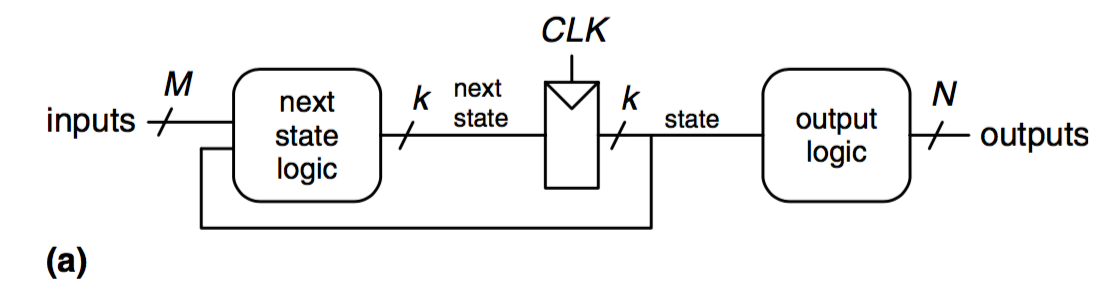
\includegraphics[width = 9cm]{images/seq/moore}
		\end{center}
		\begin{center}
				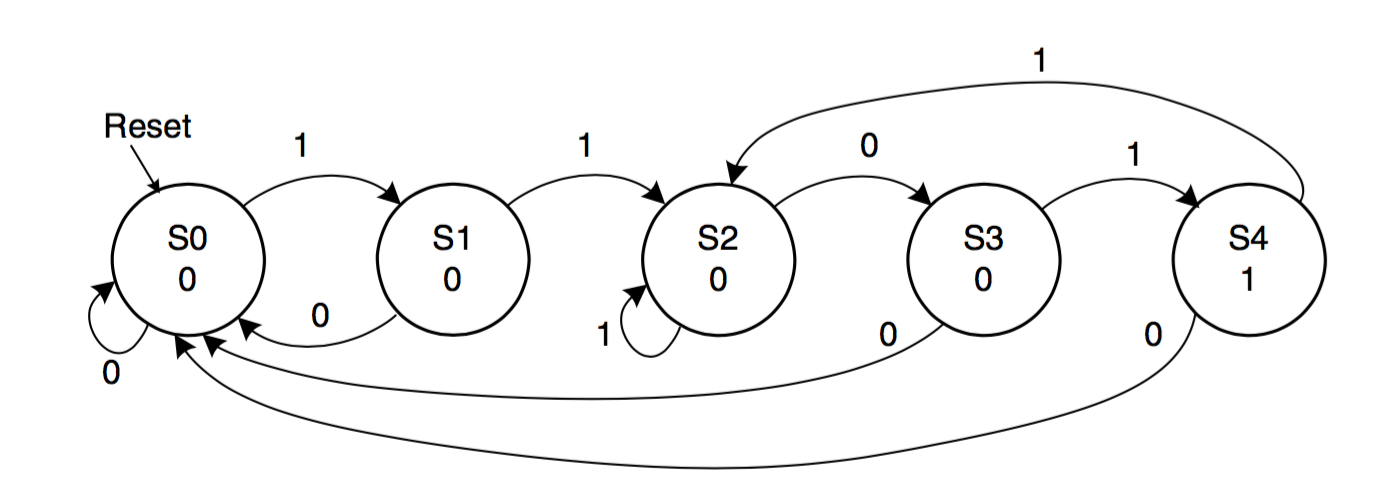
\includegraphics[width = 9cm]{images/seq/moores}
		\end{center}
		And mealy machines, where the ouputs depend on both the current state and the current inputs.
		\begin{center}
				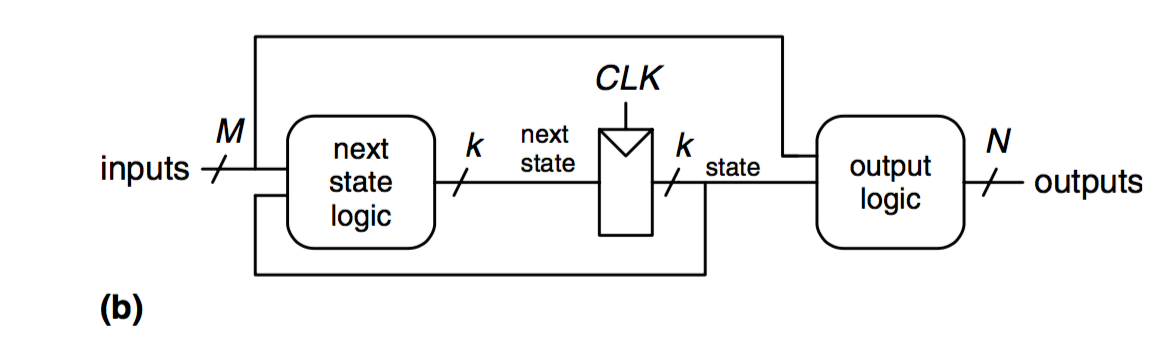
\includegraphics[width = 9cm]{images/seq/mealy}
		\end{center}
		\begin{center}
				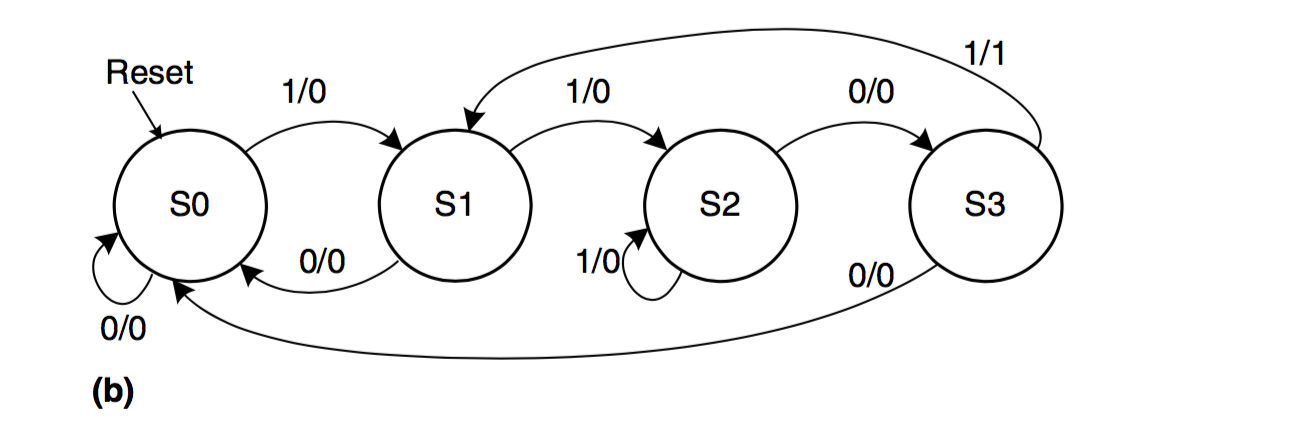
\includegraphics[width = 9cm]{images/seq/mealys}
		\end{center}
		The second picture are the transistion state diagrams, since the mealy machine also depends on the input the arcs also contain the output.\\
	To encode the different states you can use binary encoding, where each state is represented by a binary number. Or one hot encoding where each state is represented by a bit(ex 100, 010 and 001). One hot takes more place but requires fewer gates.\\
	To design a FSM:
	\begin{enumerate}
		\item Identify the inputs and outputs.
		\item Sketch a state transition diagram.
		\item For a Moore machine:
			\begin{enumerate}
				\item Write a state transition table.
				\item Write an output table.
			\end{enumerate}
		\item For a mealy machine:
			\begin{enumerate}
				\item Write a combined state transition and output table.
			\end{enumerate}
		\item Select state encodings—your selection affects the hardware design.
		\item Write Boolean equations for the next state and output logic.
		\item Sketch the circuit schematic.
	\end{enumerate}
	\paragraph{Dynamic discipline}, There is a time during which you cannot write a value to a flip-flop because it is during the clock cycle. For the circuit to sample its input correctly, the input must have stabilized at least some setup time, before the rising edge of the clock and must remain stable for at least some hold time, after the rising edge of the clock. The sum of the setup and hold times is called the aperture time of the circuit, because it is the total time for which the input must remain stable.\\The dynamic discipline states, that the inputs of a synchronous sequential circuit must be stable during the setup and hold aperture time around the clock edge.
	\paragraph{Metastable State}, when the state of the flip-flop is undefined, illegal. The flip-flop will only stay like this for some time and then change to a valid state. Metastable states are due to aschyronous input from users which we can't avoid.
	\paragraph{Synchronizer}
		A sychronizer takes an asychronous input and a clock and with a high probability returns a sychronous output.
	\subsection{Parallelism}
	\paragraph{Latency}, is the time required for a piece of information to pass from start to end of the system
	\paragraph{Throughput}, number of pieces of information the system produces per unit of time.
	\paragraph{Pipelining a circuit}, you can pipeline a circuit by adding registers into the circuit which will let you divide the calculations, like pipelining in PP. Adding a pipeline stage improves throughput at the expense of some latency.
	
	
	
	
	
	
	
	
	
	
	
	
	
	
	
	
	
	
	
	
	
	
	
	\clearpage
	
	
	
\newpage
\section{Formel-Minimierung}
	
	\begin{multicols}{2}
	
		\subsection{Karnaugh-Maps}
			\begin{center}
				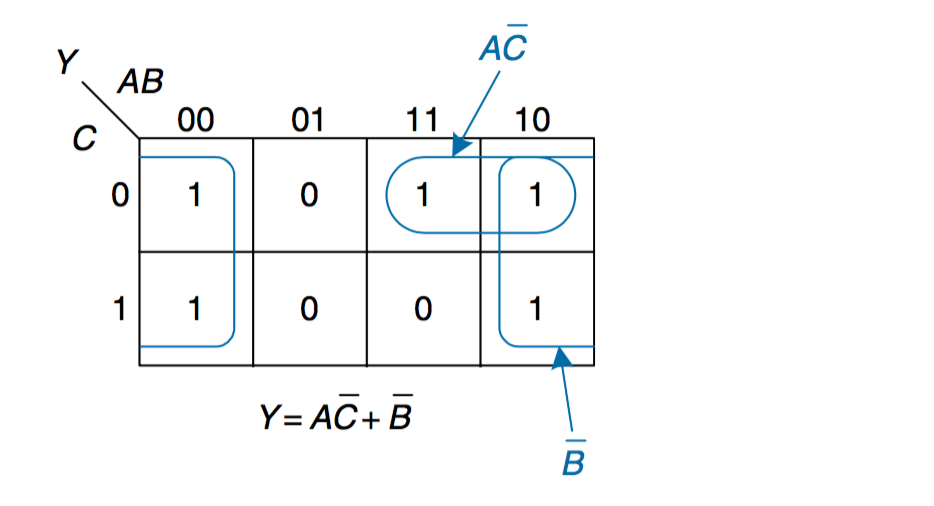
\includegraphics[width = 9cm]{images/minim/karnaugh}
			\end{center}
			You circle the biggest combination of one's possible with max length 2, and take the variables that don't change, karnaugh graphes work for functions with 4 or less variables.
		\subsection{Multiplexer}
			You can also write logic with a multiplexer. The selector of the multiplexer are your literals, the input of the multiplexer are one's for the input combination of your function, and zeros for the rest. To make the multiplexer smaller you can use a decoder.
			\paragraph{decoder}, in a decoder you make output of the multiplexer depend on a chosen literal, the High, to build a decoder it's easiest to use the truth tabel:
			\begin{center}
				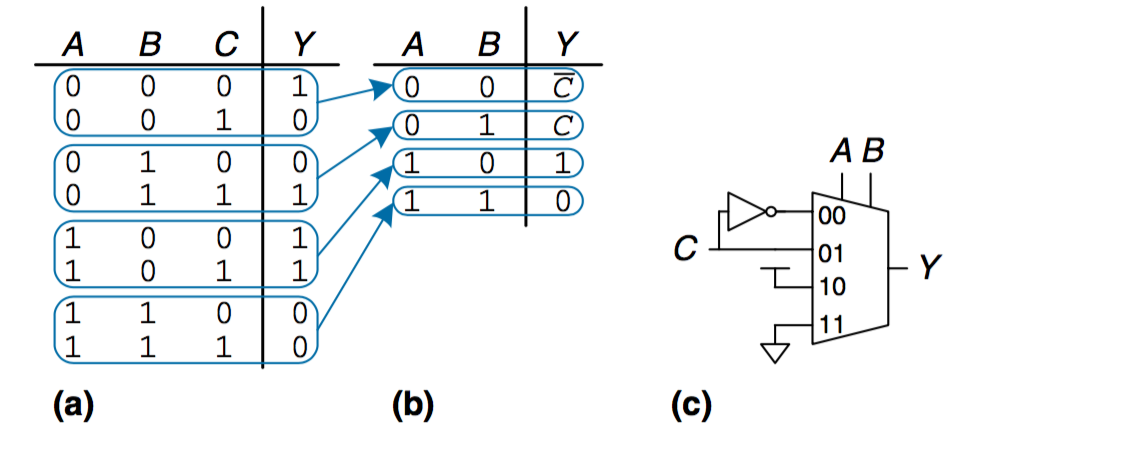
\includegraphics[width = 9cm]{images/minim/decoder}
			\end{center}			
	\end{multicols}























\newpage
\section{Assembler}

	\lstset{basicstyle=\ttfamily\scriptsize\mdseries}
	
	\begin{multicols}{2}
		\subsection{Binärzahlen}
		{\scriptsize
		\renewcommand{\arraystretch}{1.2}
		\begin{tabular}{r|c|r}
			0 & 0000 & 0 \\
			1 & 0001 & 1 \\
			2 & 0010 & 2 \\
			3 & 0011 & 3 \\
			4 & 0100 & 4 \\
			5 & 0101 & 5 \\
			6 & 0110 & 6 \\
			7 & 0111 & 7 \\
			\nop{0 & 0000 & 0 &    4 & 0100 & 4 &    8 & 1000 & 8 &    12 & 1100 & c \\
			1 & 0001 & 1 &    5 & 0101 & 5 &    9 & 1001 & 9 &    13 & 1101 & d \\
			2 & 0010 & 2 &    6 & 0110 & 6 &   10 & 1010 & a &    14 & 1110 & e \\
			3 & 0011 & 3 &    7 & 0111 & 7 &   11 & 1011 & b &    15 & 1111 & f }
		\end{tabular} \quad
		\begin{tabular}{r|c|r}
			 8 & 1000 & 8 \\
			 9 & 1001 & 9 \\
			10 & 1010 & a \\
			11 & 1011 & b \\
			12 & 1100 & c \\
			13 & 1101 & d \\
			14 & 1110 & e \\
			15 & 1111 & f 
		\end{tabular} \qquad
		\begin{tabular}{r @{ = } l}
			$2^{0}$ & 1 \\
			$2^{1}$ & 2 \\
			$2^{2}$ & 4 \\
			$2^{3}$ & 8 \\
			$2^{4}$ & 16 \\
			$2^{5}$ & 32 \\
			$2^{6}$ & 64 \\
			$2^{7}$ & 128
		\end{tabular} \quad
		\begin{tabular}{r @{ = } l}
			$2^{8}$ & 256 \\
			$2^{9}$ & 512 \\
			$2^{10}$ & 1024 \\
			$2^{11}$ & 2048 \\
			$2^{12}$ & 4096 \\
			$2^{13}$ & 8192 \\
			$2^{14}$ & 16384 \\
			$2^{15}$ & 32768
		\end{tabular}
		}
		
	\end{multicols}
	
	\subsection{Instructions}
		a = b + c\tab	add a, b, c\\
		a = b - c\tab	sub a, b, c\\
		\$s0-\$s7 \tab \$t0-\$t9\tab are memory in the SPRAM register, t are temporary(local) and s are saved.
		\begin{center}
				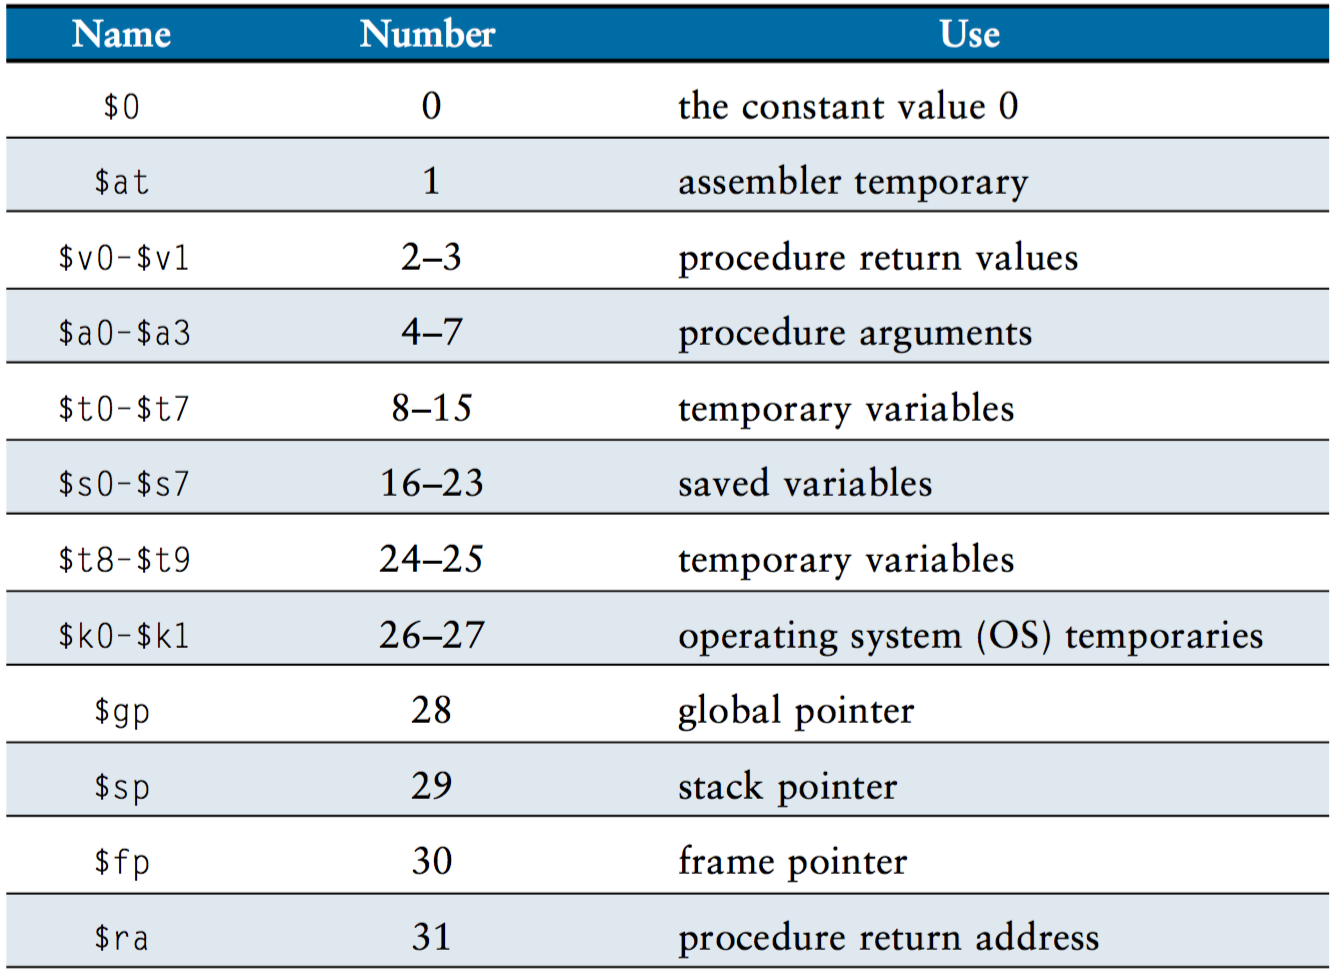
\includegraphics[width = 9cm]{images/reg}
		\end{center}
		lw \$s3, 1(\$0)\tab \#load memory word (0+1 = 1) into s3\\
		sw \$s3, 3(\$0)\tab \#write s3 into memory word 3\\
		\begin{center}
				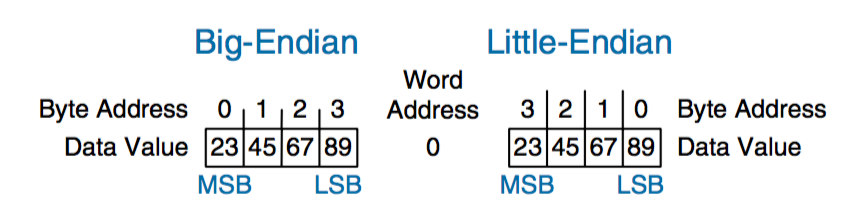
\includegraphics[width = 9cm]{images/big}
		\end{center}
		Each word in memory consists of 4 bytes, therefore you have to store in memory by a multiple of 4.\\
		addi \$s1, \$s0, -12\tab you use addi to add constants to two  register operands, there is no subi so use negative numbers instead.\\
		You can use addi to initialise a constant ex\tab addi \$s0, \$0, ox4f3c\tab initialisis \$s0 to ox4f3c
		\subsubsection{Intructions types}
		There are three instruction types R-type, I-type, and J-type. R-type instructions operate on three registers(add, sub). I-type instructions operate on two registers and a 16-bit immediate(addi,lw, sw). J-type (jump) instructions operate on one 26-bit immediate.\\Each instruction is stored in a 32 bit word. So a program consists of 32 bit numbers representing the instructions.
		\subsubsection{Logic instructions}
		R-type:\\ and s1, s2, s3\tab writes two s1 the bytes that are both 1 in s2 and s3\\
		there is also or and nor\\
		I-type: andi, ori and xori\tab they work the same as R-type but put a fix value in hexadecimal instead of last operand.
		\subsubsection{Shifts}
		Are R-type: sll(v) shift left logical, srl(v) shift right logical and sra(v) shift right arithmetic. Shifting a value left by n is like multiplying it with $2^n$. shifting a value right by n is like dividing it with $2^n$. arithmetic shifts and places one's instead of zeros.
		\subsubsection{mult in div}
		mult \$s0, \$s1\tab multiplies s0 with s1 the 32 most significant bits are placed in hi and 32 least in lo.\\
		div \$s0, \$s1\tab the qoutient is placed in lo and the remainder in hi
		\subsubsection{branching}
		if else is executed with branching and beq(branch if equal) and bne(branch if not equal) instructions.
		\begin{center}
				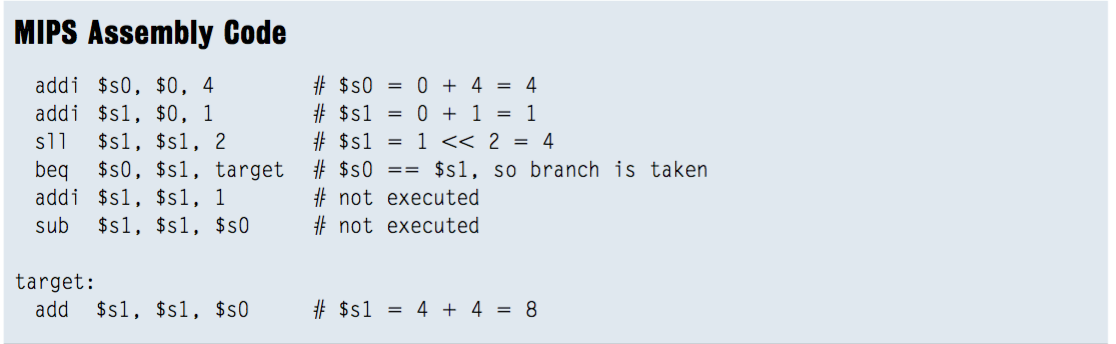
\includegraphics[width = 18cm]{images/beq}
		\end{center}
		\begin{center}
				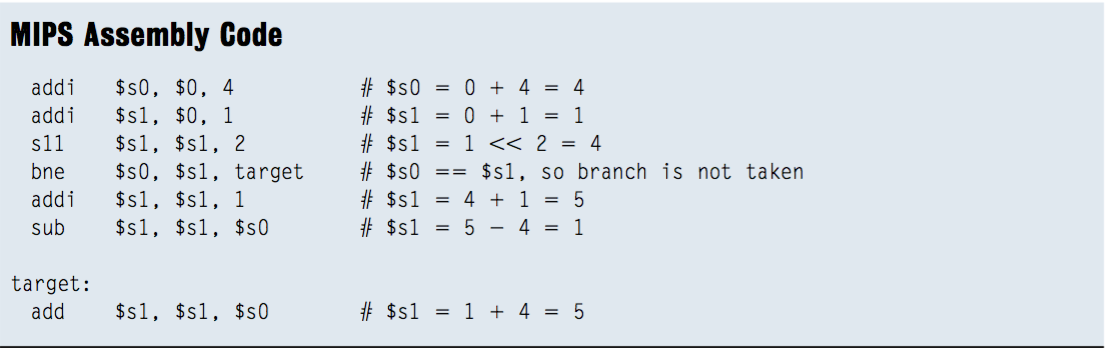
\includegraphics[width = 18cm]{images/bne}
		\end{center}
		If it's true it executes the target, else it executes the code after and then the targer.
		\subsubsection{jump}
			There are 3 jump instruction j, jr and jal. j just jumps to the specified label ex\\
			j\tab target\tab jumps to targer\\
			jr jumps to the address held in a register and jal is similar to j but is used by procedures to save a return address.
		\subsubsection{if else case}
		You can make if else statements using beq and bne:
		\begin{center}
				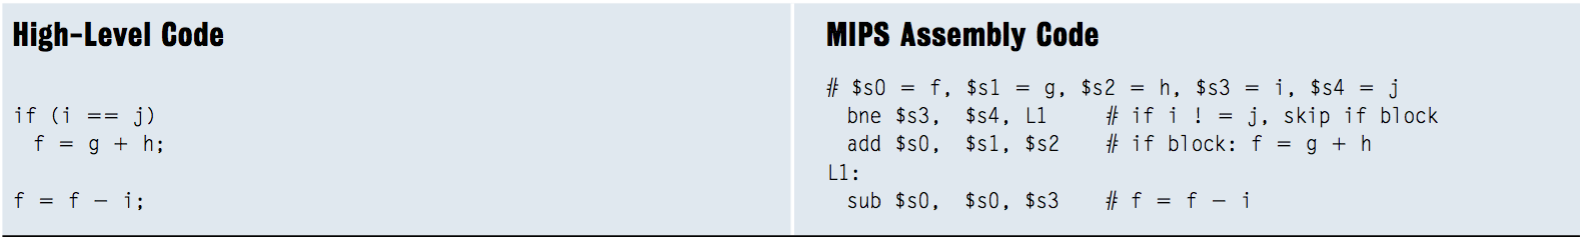
\includegraphics[width = 18cm]{images/if}
		\end{center}
		\begin{center}
				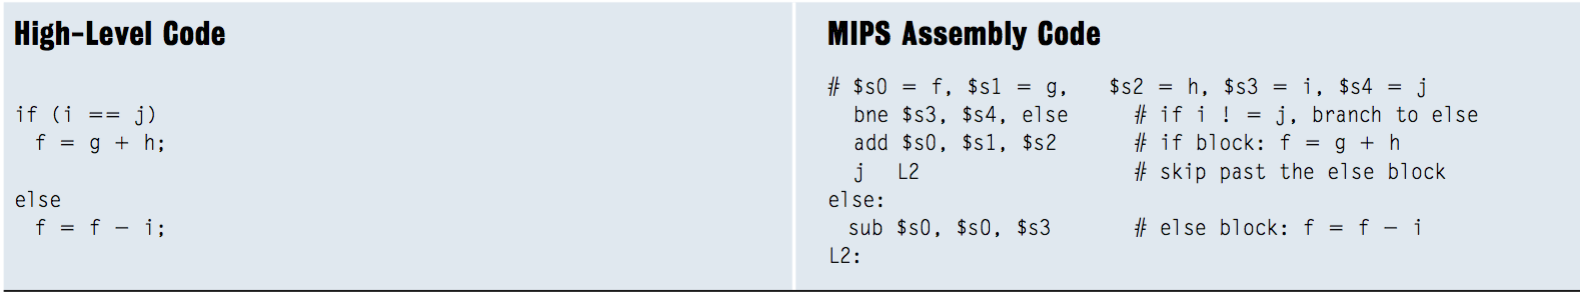
\includegraphics[width = 18cm]{images/else}
		\end{center}
		You can implement a case by using multiple if else statements.
		\begin{center}
				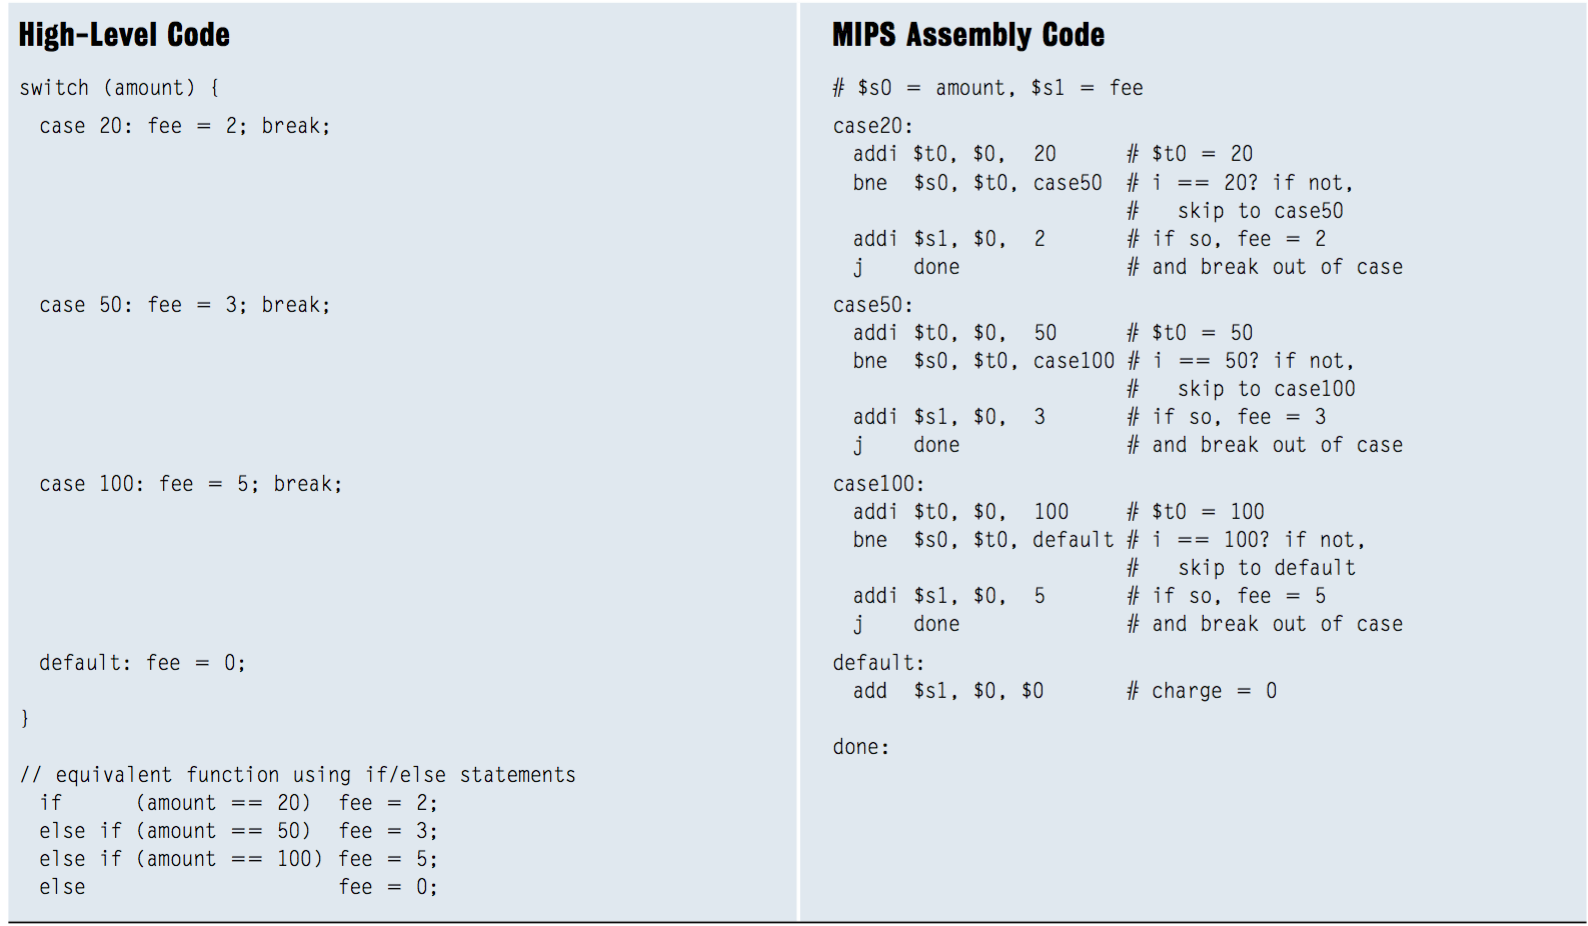
\includegraphics[width = 18cm]{images/case}
		\end{center}
		\subsubsection{Loops}
		For loops you can use the same principal as for the case but if a condition is met it will skip to the same section.
		\begin{center}
				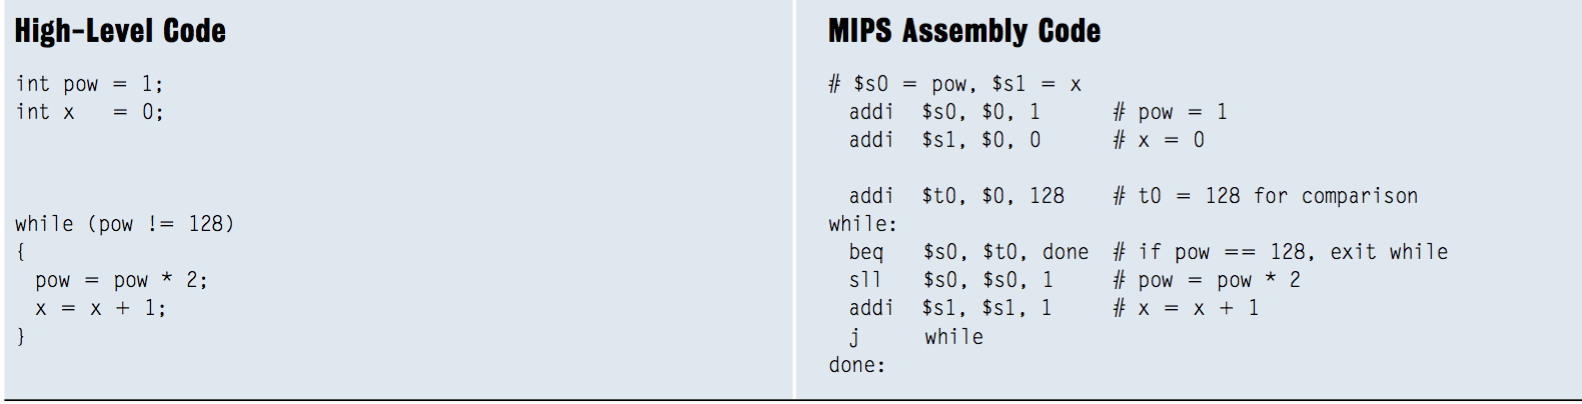
\includegraphics[width = 18cm]{images/while}
		\end{center}
		\begin{center}
				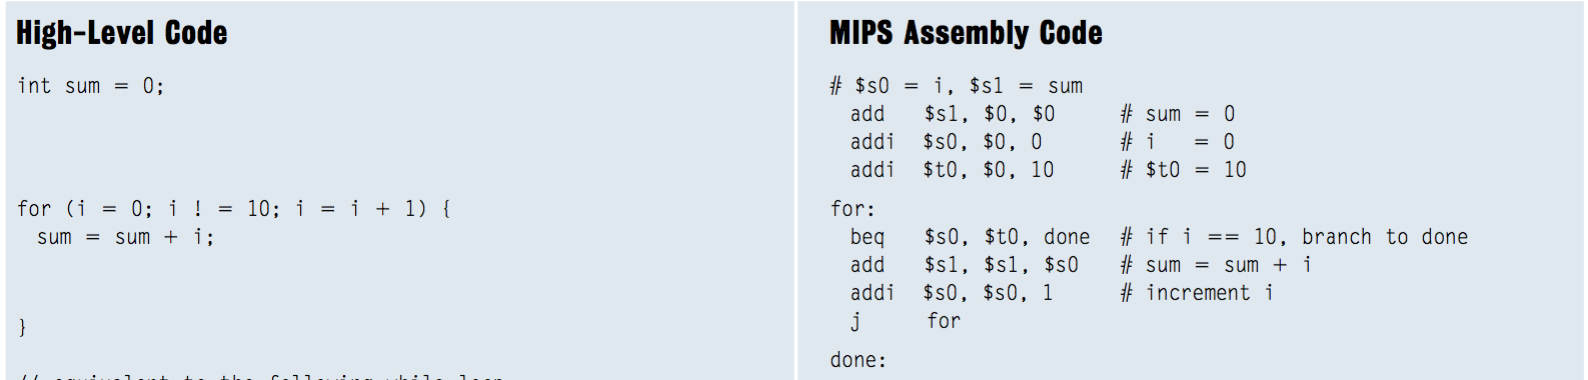
\includegraphics[width = 18cm]{images/for}
		\end{center}
		\subsubsection{magnitude comparison}
		To use a smaller than:\\
		slt rd, rs, rt\tab sets rd to 1 when rs < rt. Otherwise, rd is 0.
		\subsubsection{Arrays}
		A array is basically a address in memory which you increment by 4 to reach the other array values.
		\begin{center}
				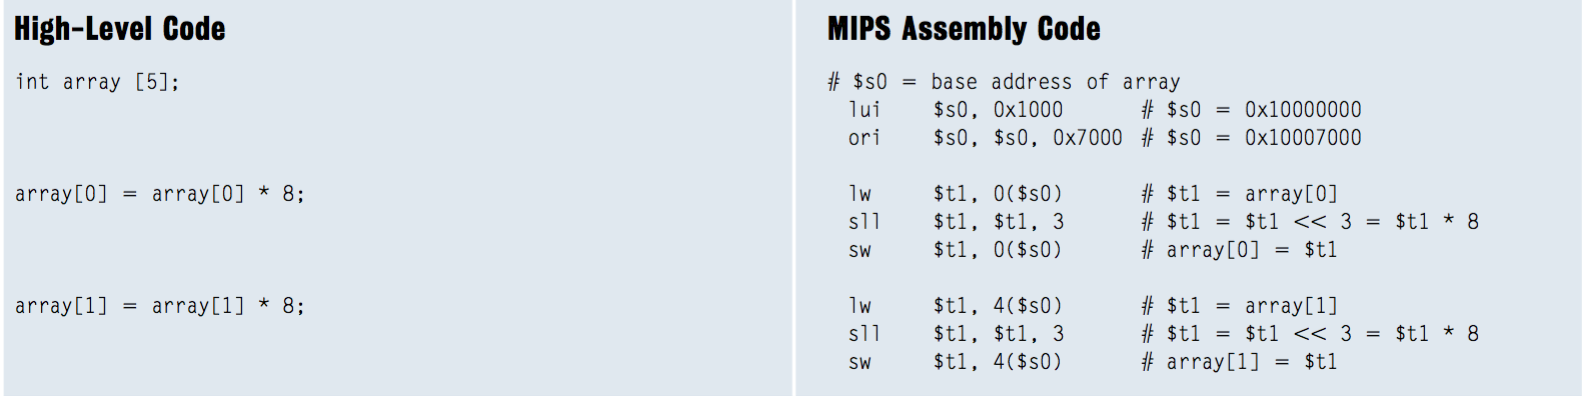
\includegraphics[width = 18cm]{images/array}
		\end{center}
		\subsubsection{Functions}
		To call a procedure jal is used and jr \$ra is used to return from a procedure. Procedures use \$a0-\$a3 as input arguments and \$v0-\$v1 as return values.
		\begin{center}
				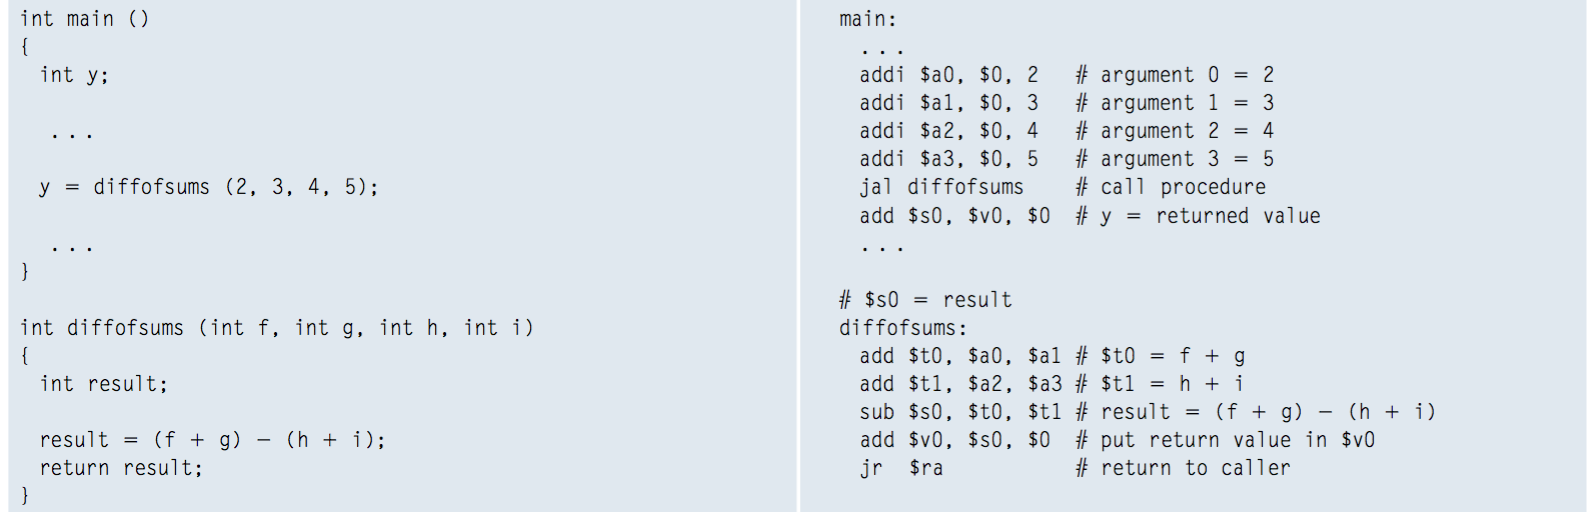
\includegraphics[width = 18cm]{images/function}
		\end{center}
		The implementation of diffofsums is not great because it changes the value of s0 which it shouldn't. To ameliorate this diffofsums should only use t variables or restore the value of s0 after the function using a stack.
		\subsubsection{stacks}
		Stacks are a LIFO queue. Better version of diffofsums using a stack:
		\begin{center}
				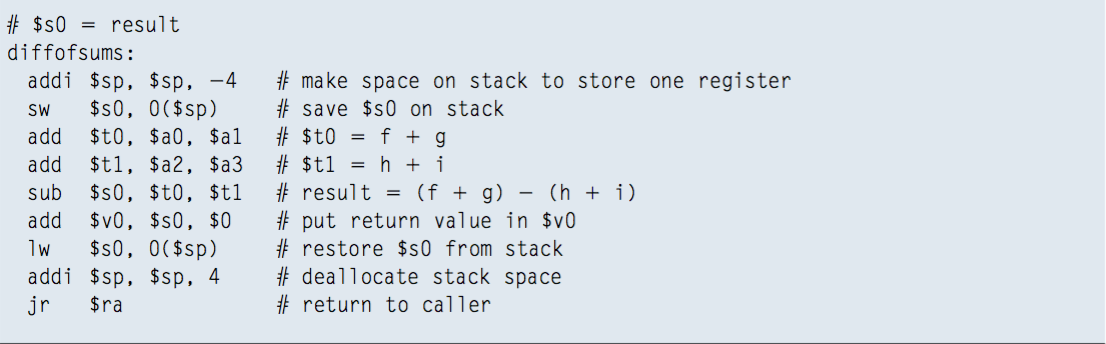
\includegraphics[width = 18cm]{images/stack}
		\end{center}
		\begin{center}
				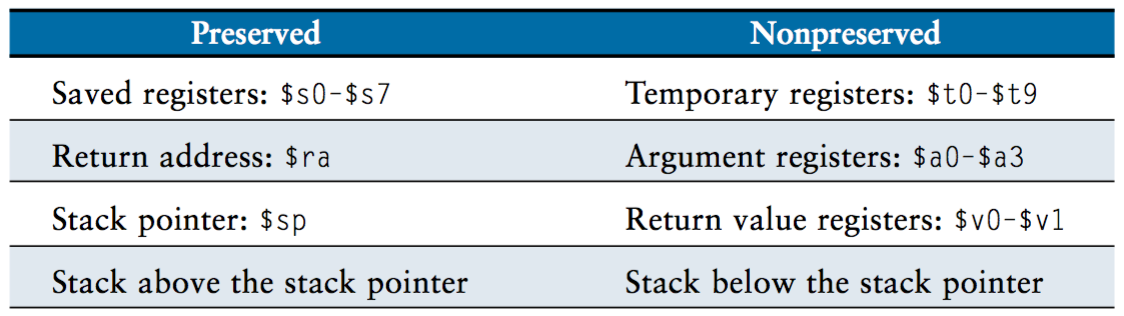
\includegraphics[width = 9cm]{images/preserved}
		\end{center}
		In recursive function calls you have to restore also non preserved registers.\\
		If more than 4 input variables are needed you can use the stack.\\
		global variables are \$gp
		\subsubsection{the Program just for interest}
		\begin{center}
				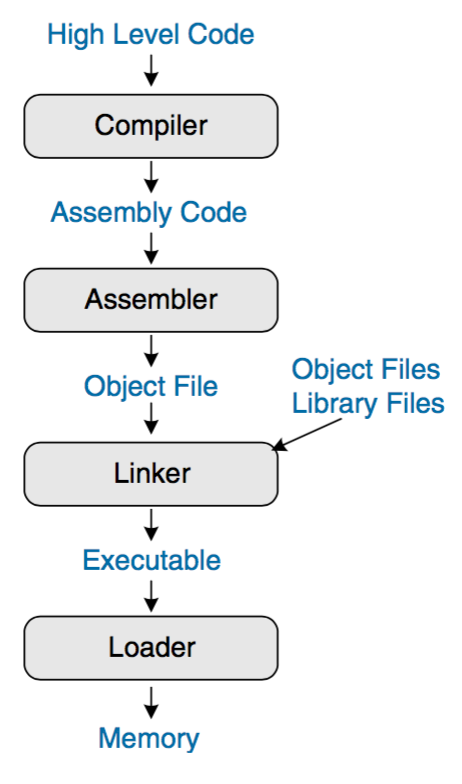
\includegraphics[height = 9cm]{images/program}
		\end{center}
		


\newpage
\section{Verilog}
	\lstset{language=Verilog}
	\lstset{basicstyle=\ttfamily\mdseries}
	\begin{multicols}{2}
	
	\subsection{Operatoren}
		\begin{tabular}{ll}
		\lstinline!+!, \lstinline!-!, \lstinline!*! & Arithmetic operators \\
		\lstinline*/ * &  Integer division (fractional part truncated) \\
		\lstinline*%* &  Modulo (takes sign of the first operand) \\
		\lstinline!**! &  Exponent \\
		\lstinline*-* & Negation (2's complement) \\
		\\
		\lstinline*~* & Bitwise NOT (1's complement) \\
		\lstinline*&* & Bitwise AND \\
		\lstinline*|* & Bitwise OR \\
		\lstinline*^* & Bitwise XOR \\
		\lstinline*^~*, \lstinline*~^* & Bitwise XNOR \\ 
		\\
		\lstinline*<<*, \lstinline*>>* & Logical shift (padding with 0) \\
		\lstinline*<<<*, \lstinline*>>>* & Arithmetic shift (padding with leftmost \\
		& bit when shifting right) \\ 
		\lstinline*?:* & Conditional \\
		\lstinline*{ a, b }* & Concatenation \\
		\lstinline*{ num { a }}* & Replication \\
		\end{tabular} 
	
	\subsection{Vergleiche}
		\begin{tabular}{ll}
		\lstinline*>*, \lstinline*<*, \lstinline*>=*, \lstinline*<=* & 	Relational operators (\lstinline*0*, \lstinline*1* or \lstinline*x*) \\
		\lstinline*==*, \lstinline*==* & Logical equality (\lstinline*0*, \lstinline*1* or \lstinline*x*) \\
		\lstinline*===*, \lstinline*!==* & Case equality (\lstinline*0* or \lstinline*1*) \\
		\end{tabular}
	
	
	\subsection{Konstanten}
		Angabe mit [\textless width in bits\textgreater]'\textless base\textgreater\textless number\textgreater \\
		\begin{tabular}{ll}
		\lstinline*'b* &(binär, 2) \\
		\lstinline*'o* &(oktal, 8) \\
		\lstinline*'d* &(dezimal, 10) \\
		\lstinline*'h* &(hexadezimal, 16)
		\end{tabular} \\
		z.B. \lstinline*-4'd3* (\lstinline*1101*), \lstinline*4'b11* (\lstinline*0011*), \lstinline*'h08FF* (16 bit hex)
		
	
	
	\subsection{Module}
	\lstset{basicstyle=\ttfamily\scriptsize\mdseries}
	In Verilog bestehen die Modelle aus Modulen, wobei jedes Modul ein Interface besitzt, welches die Inputs und Outputs definiert.
	Ein Modul kann dann instanziert werden, wobei ihm ein eindeutiger Name zugewiesen wird.
		\begin{lstlisting}[language=Verilog]
// modul definieren
module abc(input a,b, input [3:0] data, output out);
	wire x;
	assign x = (!a || b) ^ a;
	assign out = x ;
endmodule

// module instanzieren
module main(..)
	abc A1(a,x,data,myvar);
endmodule
		\end{lstlisting}
	
	\vfill
	
	\subsection{always}
	\lstset{basicstyle=\ttfamily\normalsize\mdseries}
	Mit \lstinline+always+ lassen sich Endlosschleifen ausdrücken. Zusätzlich
	kann die Ausführung auf positive/negative Flanken einer bestimmten Variable
	eingeschränkt werden.
	\lstset{basicstyle=\ttfamily\scriptsize\mdseries}
		\begin{lstlisting}[language=Verilog]
always @([posedge | negedge] var) begin .. end
		\end{lstlisting}
	
		
	\subsection*{Zeitauflösung/Delays}
	\lstset{basicstyle=\ttfamily\normalsize\mdseries}
	\begin{tabular}{lp{7.3cm}}
		\lstinline+'timescale <Zeiteinheit>/<Aufloesung>+ &
	\end{tabular}
	Wird im Header eines Moduls angegeben. z.B. \lstinline+1ns/100ps+ bedeutet dass der Delay-Operator \lstinline+#1+ für 1ns verzögert und die Simulation in 100ps Zeitschritten läuft. 
			
	\subsection*{Zuweisungsoperatoren}
	\lstset{basicstyle=\ttfamily\normalsize\mdseries}
	\begin{tabular}{lp{6.5cm}}
		\lstinline+a = b+   &   \emph{blocking assignment}: Der Wert der Zielvariable wird sofort aktualisiert. \\
		\lstinline+a <= b+   &   \emph{non-blocking assignment}: Die rechte Seite wird	
	sofort ausgewertet, die Zuweisung erfolgt jedoch erst im nächsten Zeitschritt (nicht Flanke/Takt!), was eine parallele
	Ausführung solcher Befehle ermöglicht. Die NBA's bewirken keine Verzögerung im Timingdiagramm (ausser wenn die Auflösung
	gleich der Zeiteinheit ist, was nicht sehr sinnvoll ist). \\
		\lstinline+assign a = b+ & \emph{continuous assignment}: Weist der Zielvariable sofort den Wert des Ausdrucks zu, wenn immer dieser ändert. Ausserhalb von always und initial Blöcken!
	\end{tabular}
	
	
	\subsection*{Weitere Konstrukte}
	\lstset{basicstyle=\ttfamily\normalsize\mdseries}
	\begin{tabular}{lp{5cm}}
		\lstinline+reg a,b;+   &   Lokale 1-Bit Variablen (Register) \\
		\lstinline+reg [3:0] d;+   &   Lokale 4-Bit Variablen \\
		\lstinline+wire a+   &   Draht, verbindet z.B. Ein-/Ausgänge von Modulen \\
		\lstinline+assign #3 a = b & c+   &   Zuweisung (Delay: 3 Einheiten) \\
	\end{tabular}
	
	
	\end{multicols}
	
	
\newpage
\section{mips Processor}
	A computer architecture is defined by it's instruction set and architectural state. The architectural state for the MIPS processor consists of the program counter and the 32 registers. We only consider the following instruction set:\\ R-type arithmetic/logic instructions: add, sub, and, or, slt.\\
	Memory instructions: lw, sw\\
	Branches: beq\\
	After having built the microarchitectures with these instructions we extend them with addi and j.\\
	We will divide our microarchitectures into two interacting parts: the datapath and the control. The datapath operates on words of data. It contains structures such as memories, registers, ALUs, and multiplexers. MIPS is a 32-bit architecture, so we will use a 32-bit datapath. The control unit receives the current instruction from the datapath and tells the datapath how to execute that instruction. Specifically, the control unit produces multiplexer select, register enable, and memory write signals to control the operation of the datapath.\\
	It is often good to seperate the memory into two, one containing the instructions and the other the data.\\
	The microprocessor is built of clocked state elements and combinational logic, so it too is a synchronous sequential circuit. Indeed, the processor can be viewed as a giant finite state machine, or as a collection of simpler interacting state machines.\\
	\subsection{Execution time}
	The execution time for a program is given by:
	\begin{equation}
		T= (\#instructions)*(\frac{cycles}{instruction})(\frac{seconds}{cycle})
	\end{equation}
	\subsection{Different architectures}
		\subsubsection{Singel-sycle}
			Executes an entire instruction in one cycle. It is easy to explain and has a simple control unit. Because it completes the operation in one cycle, it does not require any nonarchitectural state. However, the cycle time is limited by the slowest instruction.
			\begin{center}
				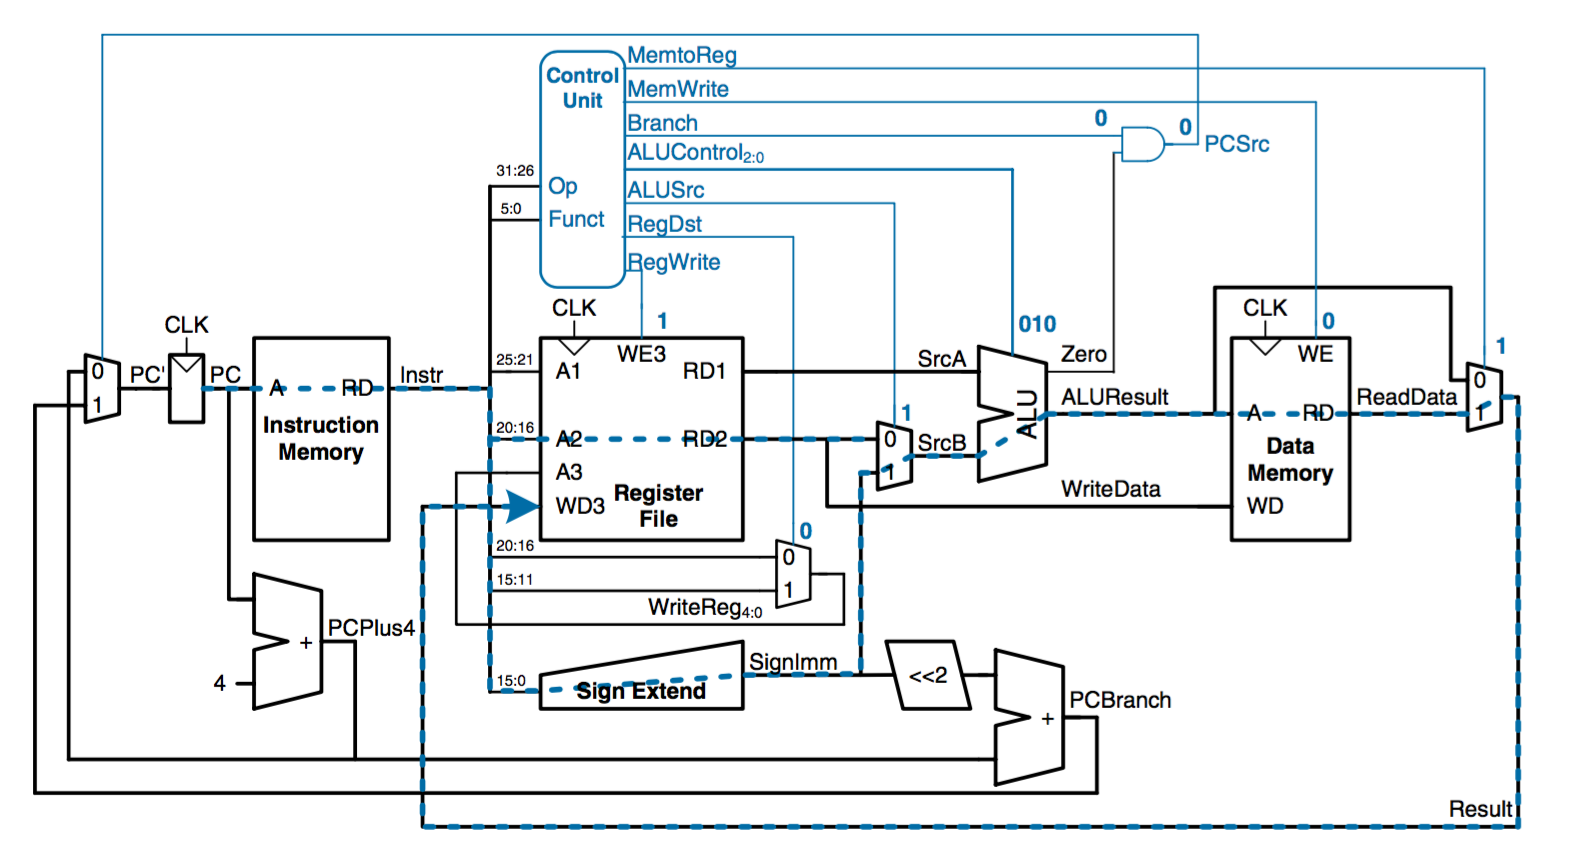
\includegraphics[width = 15cm]{images/single.png}
			\end{center}
			\paragraph{Performance}
			\begin{equation}
				T_c = T_{pcq_PC} + 2*t_{mem} + t_{RFread} + 2*t_{mux} + t_{ALU} + t_{RFsetup}
			\end{equation}
			\paragraph{Problems}
				The single cycle has 3 major problems:
				\begin{enumerate}
					\item requires a clock cycle long enough to support the slowest instruction (lw)
					\item requires 3 adders which are expensive
					\item Has two memories one for instructions and one for data. Most computers have one.
				\end{enumerate}
		\subsubsection{Multicycle}
			executes instructions in a series of shorter cycles. In each short step, the processor can read or write the memory or register file or use the ALU. Simpler instructions execute in fewer cycles than complicated ones. Moreover, the multicycle microarchitecture reduces the hardware cost by reusing expensive hardware blocks such as adders and memories(has one adder and one memory). The multicycle microprocessor accomplishes this by adding several nonarchitectural registers to hold intermediate results. The multicycle processor executes only one instruction at a time, but each instruction takes multiple clock cycles. The controller produces different signals on different steps during execution of a single instruction, so it is now a finite state machine rather than combinational logic.
			\begin{center}
				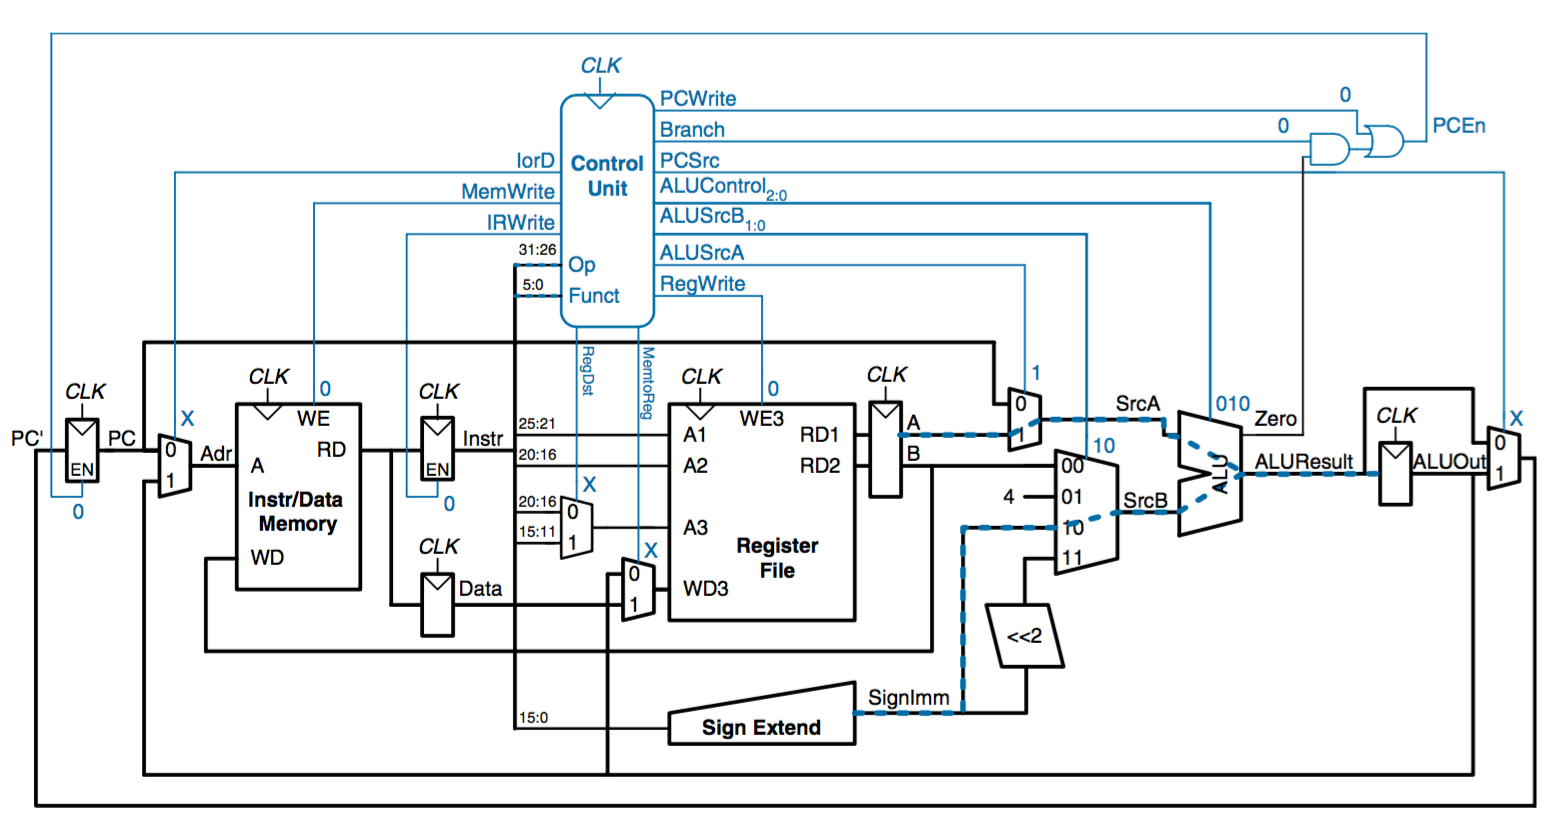
\includegraphics[width = 15cm]{images/multi}
			\end{center}
			\paragraph{Performance}
			The multicycle processor requires three cycles for beq and j instruc- tions, four cycles for sw, addi, and R-type instructions, and five cycles for lw instructions. The CPI depends on the relative likelihood that each instruction is used.
			\begin{equation}
				T_c = T_{pcq} + t_{mux} + MAX(t_{ALU}+ t_{mux}, t_{mem})+ t_{setup}
			\end{equation}
		\subsubsection{Pipeline}
			applies pipelining to the single-cycle microarchitecture. It therefore can execute several instructions simultaneously, improving the throughput significantly. Pipelining must add logic to handle dependencies between simultaneously executing instructions. It also requires nonarchitectural pipeline registers. The added logic and registers are worthwhile; all commercial high-performance processors use pipelining today.\\
			We design a pipelined processor by sub- dividing the single-cycle processor into five pipeline stages. Thus, five instructions can execute simultaneously, one in each stage. Because each stage has only one-fifth of the entire logic, the clock frequency is almost five times faster. Hence, the latency of each instruction is ideally unchanged, but the throughput is ideally five times better. Microprocessors execute millions or billions of instructions per second, so throughput is more important than latency.  Pipelining introduces some overhead, so the throughput will not be quite as high as we might ideally desire.\\
			Reading and writing the memory and register file and using the ALU typically constitute the biggest delays in the processor. We choose five pipeline stages so that each stage involves exactly one of these slow steps. Specifically, we call the five stages Fetch, Decode, Execute, Memory, and Writeback. They are similar to the five steps that the multicycle processor used to perform lw. In the Fetch stage, the processor reads the instruction from instruction memory. In the Decode stage, the processor reads the source operands from the register file and decodes the instruction to produce the control signals. In the Execute stage, the processor performs a computation with the ALU. In the Memory stage, the processor reads or writes data memory. Finally, in the Writeback stage, the processor writes the result to the register file, when applicable.
			\begin{center}
				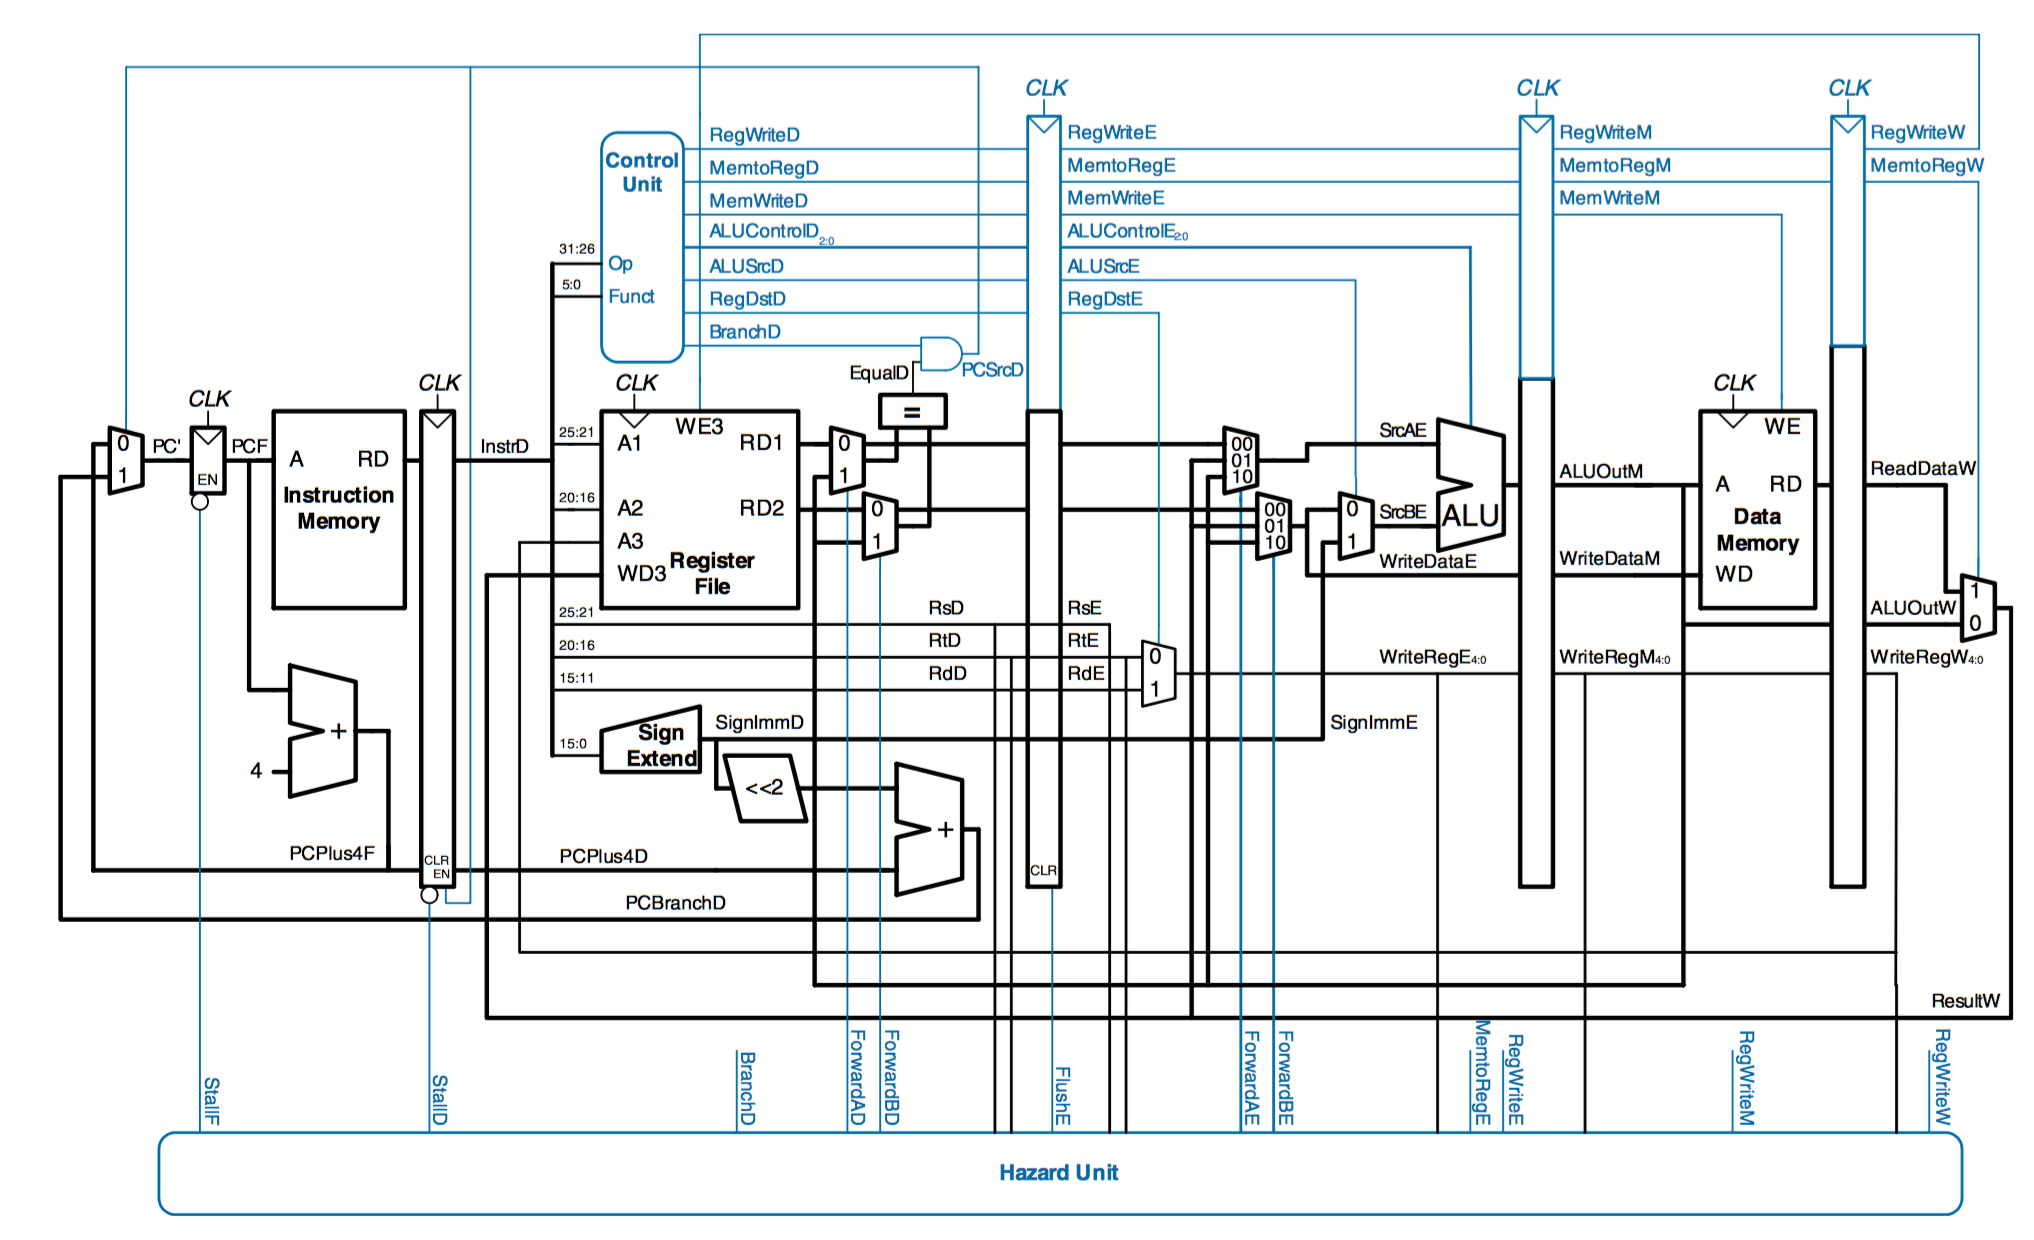
\includegraphics[width = 15cm]{images/pipeline}
			\end{center}
			\paragraph{Hazards}
				Hazards are classified as data hazards or control hazards. A data hazard occurs when an instruction tries to read a register that has not yet been written back by a previous instruction. A control hazard occurs when the decision of what instruction to fetch next has not been made by the time the fetch takes place. This can kind of be fixed with the hazard detection unit(by forwarding). They can also be solved by stalling the pipeline. stalling a stage is performed by disabling the pipeline register, so that the contents do not change. When a stage is stalled, all previous stages must also be stalled, so that no subsequent instructions are lost. Stalls degrade performance.
			\paragraph{Performance}
				CPI should idealy be 1, but a stall or a flush waste a cycle.



















=
	
\newpage
\section{Memory}
	Computer performance depends on the speed of the memory and the processor. DRAM (dynamic ram)is 10 to 100 times slower than processors.\\
	Computer memories are the combination of a small fast cheap memory and a slow large cheap memory. The cache is SRAM(static)(main memory). A cache hit is when memory is retrieved from the SRAM or it's a cache miss. The third level of memory is the hard disk(virtual memory).\\
	cache is physical memory. main memory. virtual.
	\paragraph{Average memory access time (AMAT)}
	\begin{equation}
		AMAT = t_{cache}+ MR_{cache}(t_{MM} + MR_{MM}t_{VM})
	\end{equation}
	MR= miss rate\\
	If a cache misses the data found will be copied to the cache.\\
	Two rules for what is in the cache: spatial and temporal locality. Spatial, means that when a word is copied to the cache it can also copy similar words. Temporal, means that if there is a cache miss that data will be copied to the cache because it might be searched for again.
	\subsection{Caches}
		Caches are organized as two-dimensional arrays. The rows are called sets, and the columns are called ways. Each entry in the array consists of a data block and its associated valid and tag bits. Caches are characterized by:
		\begin{enumerate}
			\item capacity C
			\item block size B and number of blocks, B = C/b
			\item number of blocks in a set N
		\end{enumerate}
	\subsection{Types of cache}
	\paragraph{Direct mapped cache}
		Each set in the cache contains one block(one data per address). Block one of main memory maps to the set 1 of the cache and so on until the last set in the cache, then the next block in MM maps to the first set in the cache again.
	\paragraph{N-way set}
		Each set contains N blocks. Have lower miss rates, but are slower and more expensive.
	\paragraph{fully associative} is a cache with only one set(B-way set).\\
	If a set is full when new data must be loaded, most of the time LRU(least recently used) block is deleted.
	\subsection{Multiple level caches}
	Most systems use multiple levels of caches. Each level is also from SPRAM but bigger and therefore slower.
	\subsection{Misses}
	The first request to a cache block is called a compulsory miss, because the block must be read from memory regard- less of the cache design. Capacity misses occur when the cache is too small to hold all concurrently used data. Conflict misses are caused when several addresses map to the same set and evict blocks that are still needed.
	
	
	\begin{multicols}{2}
		\subsection{Kaskadierung von RAM-Chips}
			\begin{center}
				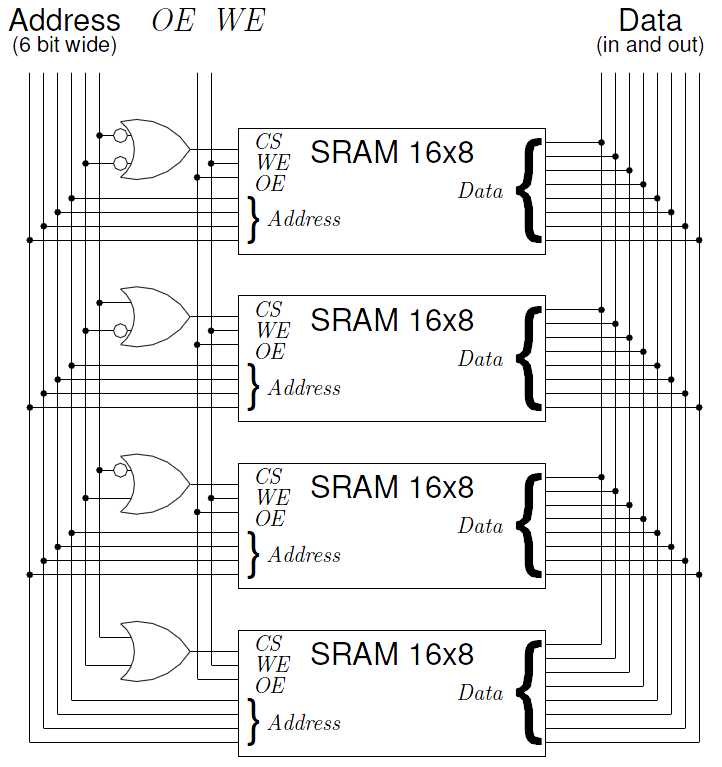
\includegraphics[width = 7cm]{images/mem/mem1.png}
			\end{center}
		ram looses it's memory when the power is turned off rom doesn't.
		
		
		\subsection{64 KBit (4096x16)}
			\begin{center}
			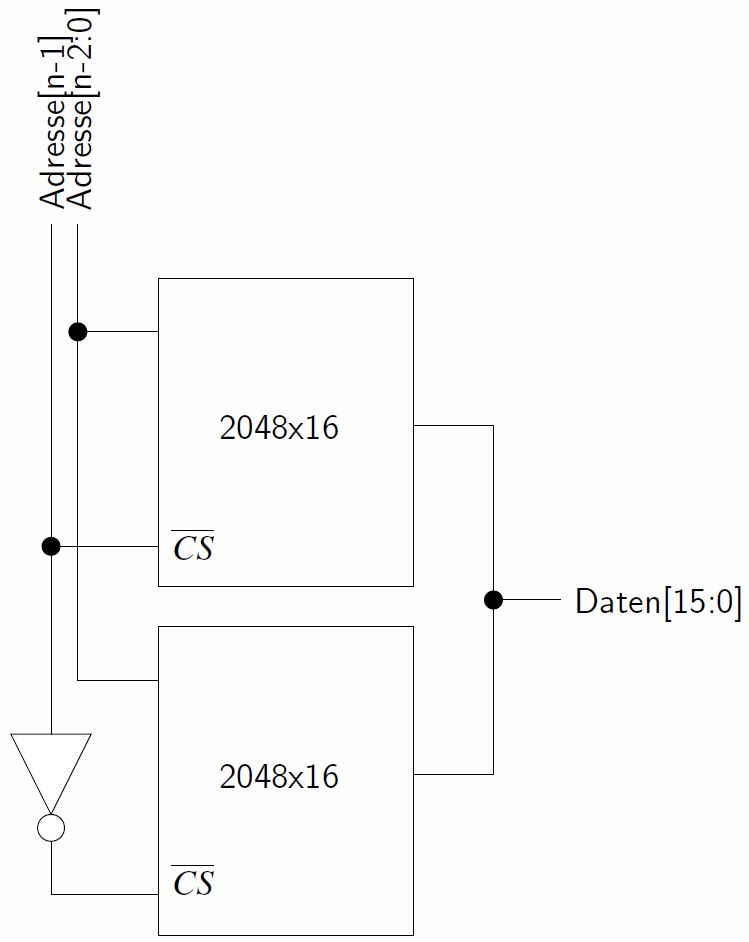
\includegraphics[width = 6cm]{images/mem/mem2-1.png}
			\end{center}
			
		\subsection{64 KBit (2048x32)}
			\begin{center}
			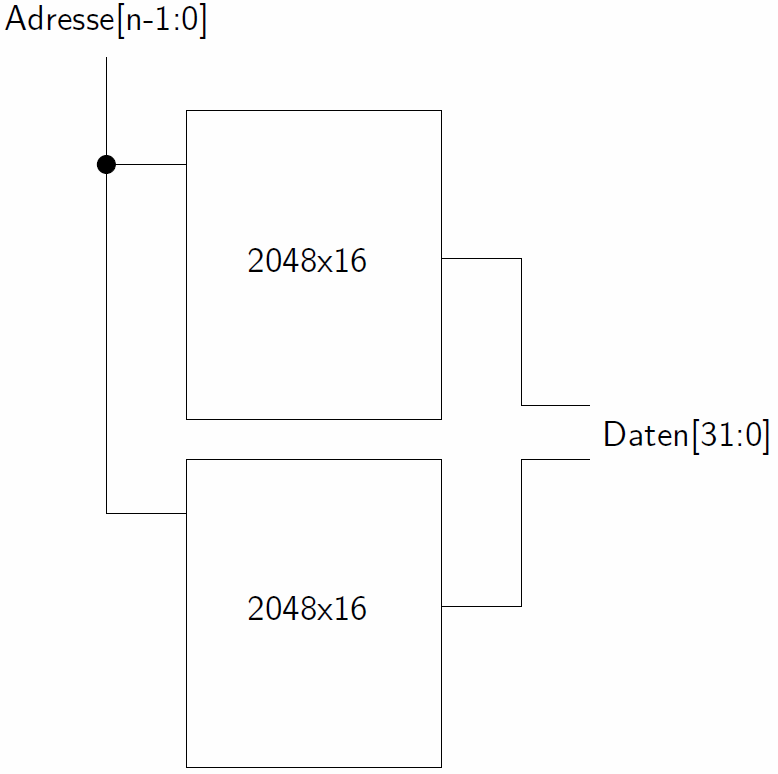
\includegraphics[width = 6cm]{images/mem/mem2-2.png}
			\end{center}
		
		\subsection{128 KBit (4096x32)}
			\begin{center}
			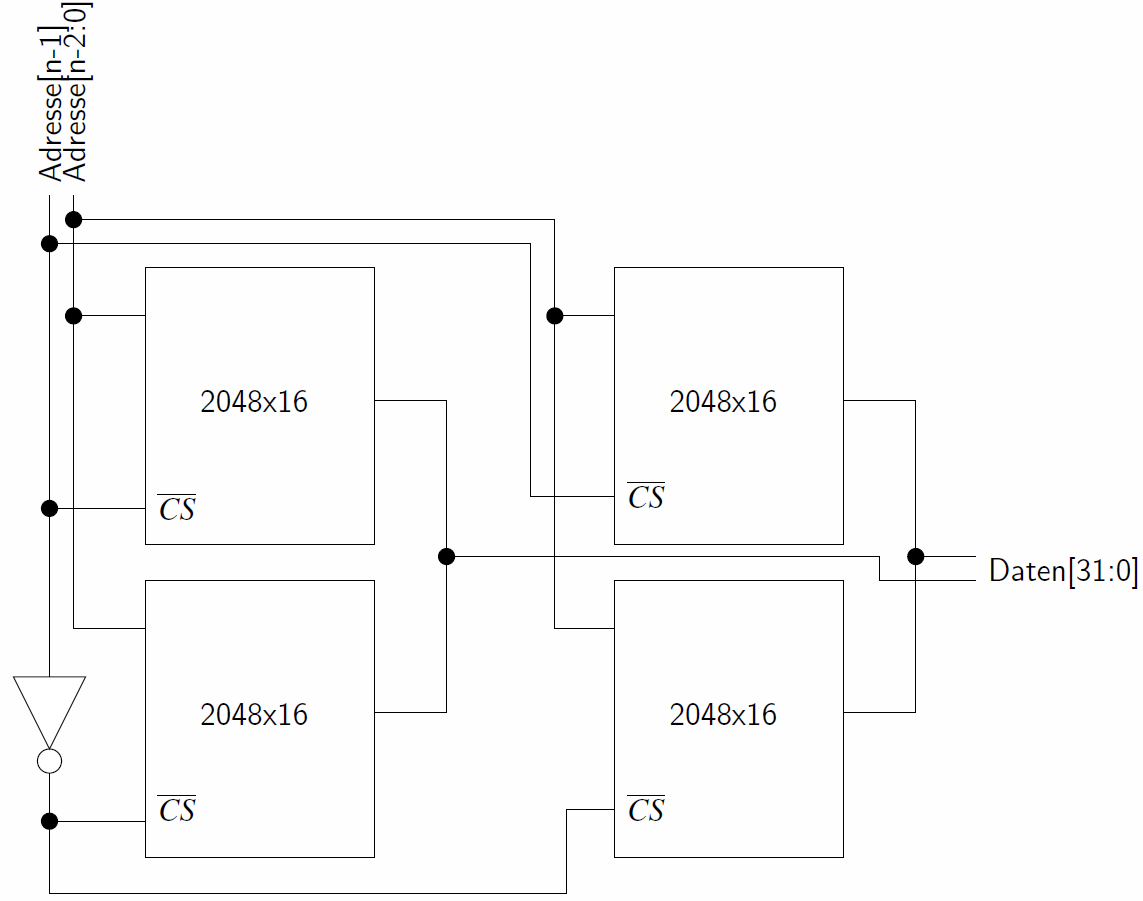
\includegraphics[width = 9cm]{images/mem/mem2-3.png}
			\end{center}
		

	\end{multicols}

	
\section{CMOS}
	\begin{multicols}{2}
			Es gibt zwei Schalttypen, NMOS und PMOS, beide werden aus Halbleitertransistoren aufgebaut.
			Dabei kommt dotiertes Silizium zum Einsatz, entweder p-dotiert (mit einem Überschuss an positiver Ladung)
			oder n-dotiert (zu viel negative Ladung).
			
			PMOS und NMOS Schalter dürfen nicht beliebig verbaut werden, ein NMOS-Transistor funktioniert nur zwischen
			\verb+out+ und \verb+GND+, während ein PMOS-Transistor nur zwischen \verb+VDD+ und \verb+out+ eingesetzt werden darf.
			
			\begin{center}
			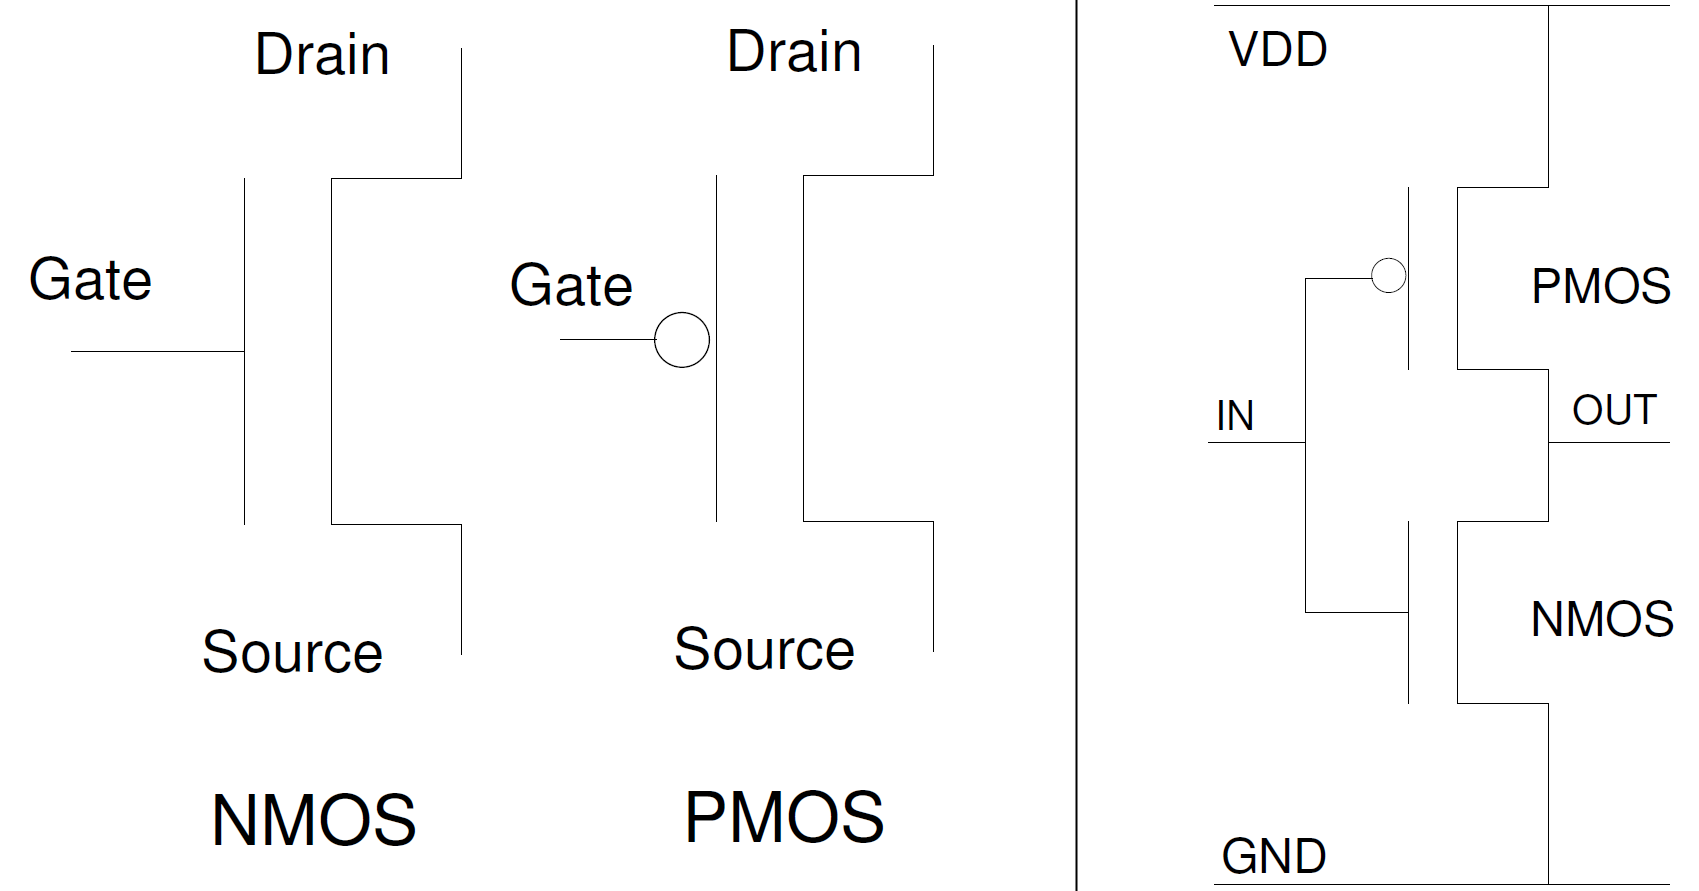
\includegraphics[width = 8cm]{images/mem/cmos.png}
			\end{center}
	\end{multicols}



















\newpage
\section{Binärzahlen (2er-Komplement)}
	\begin{center}
	{ \small
	\begin{tabular}{| rrr | rrr | rrrr | rrrr |}
		
						\hline
			00000000 & 0 & 0x00 & 01000000 & 64 & 0x40 & 11111111 & -1 & 255 & 0xff & 10111111 & -65 & 191 & 0xbf \\
			00000001 & 1 & 0x01 & 01000001 & 65 & 0x41 & 11111110 & -2 & 254 & 0xfe & 10111110 & -66 & 190 & 0xbe \\
			00000010 & 2 & 0x02 & 01000010 & 66 & 0x42 & 11111101 & -3 & 253 & 0xfd & 10111101 & -67 & 189 & 0xbd \\
			00000011 & 3 & 0x03 & 01000011 & 67 & 0x43 & 11111100 & -4 & 252 & 0xfc & 10111100 & -68 & 188 & 0xbc \\
			00000100 & 4 & 0x04 & 01000100 & 68 & 0x44 & 11111011 & -5 & 251 & 0xfb & 10111011 & -69 & 187 & 0xbb \\
			00000101 & 5 & 0x05 & 01000101 & 69 & 0x45 & 11111010 & -6 & 250 & 0xfa & 10111010 & -70 & 186 & 0xba \\
			00000110 & 6 & 0x06 & 01000110 & 70 & 0x46 & 11111001 & -7 & 249 & 0xf9 & 10111001 & -71 & 185 & 0xb9 \\
			00000111 & 7 & 0x07 & 01000111 & 71 & 0x47 & 11111000 & -8 & 248 & 0xf8 & 10111000 & -72 & 184 & 0xb8 \\
			\hline
			00001000 & 8 & 0x08 & 01001000 & 72 & 0x48 & 11110111 & -9 & 247 & 0xf7 & 10110111 & -73 & 183 & 0xb7 \\
			00001001 & 9 & 0x09 & 01001001 & 73 & 0x49 & 11110110 & -10 & 246 & 0xf6 & 10110110 & -74 & 182 & 0xb6 \\
			00001010 & 10 & 0x0a & 01001010 & 74 & 0x4a & 11110101 & -11 & 245 & 0xf5 & 10110101 & -75 & 181 & 0xb5 \\
			00001011 & 11 & 0x0b & 01001011 & 75 & 0x4b & 11110100 & -12 & 244 & 0xf4 & 10110100 & -76 & 180 & 0xb4 \\
			00001100 & 12 & 0x0c & 01001100 & 76 & 0x4c & 11110011 & -13 & 243 & 0xf3 & 10110011 & -77 & 179 & 0xb3 \\
			00001101 & 13 & 0x0d & 01001101 & 77 & 0x4d & 11110010 & -14 & 242 & 0xf2 & 10110010 & -78 & 178 & 0xb2 \\
			00001110 & 14 & 0x0e & 01001110 & 78 & 0x4e & 11110001 & -15 & 241 & 0xf1 & 10110001 & -79 & 177 & 0xb1 \\
			00001111 & 15 & 0x0f & 01001111 & 79 & 0x4f & 11110000 & -16 & 240 & 0xf0 & 10110000 & -80 & 176 & 0xb0 \\
			\hline
			00010000 & 16 & 0x10 & 01010000 & 80 & 0x50 & 11101111 & -17 & 239 & 0xef & 10101111 & -81 & 175 & 0xaf \\
			00010001 & 17 & 0x11 & 01010001 & 81 & 0x51 & 11101110 & -18 & 238 & 0xee & 10101110 & -82 & 174 & 0xae \\
			00010010 & 18 & 0x12 & 01010010 & 82 & 0x52 & 11101101 & -19 & 237 & 0xed & 10101101 & -83 & 173 & 0xad \\
			00010011 & 19 & 0x13 & 01010011 & 83 & 0x53 & 11101100 & -20 & 236 & 0xec & 10101100 & -84 & 172 & 0xac \\
			00010100 & 20 & 0x14 & 01010100 & 84 & 0x54 & 11101011 & -21 & 235 & 0xeb & 10101011 & -85 & 171 & 0xab \\
			00010101 & 21 & 0x15 & 01010101 & 85 & 0x55 & 11101010 & -22 & 234 & 0xea & 10101010 & -86 & 170 & 0xaa \\
			00010110 & 22 & 0x16 & 01010110 & 86 & 0x56 & 11101001 & -23 & 233 & 0xe9 & 10101001 & -87 & 169 & 0xa9 \\
			00010111 & 23 & 0x17 & 01010111 & 87 & 0x57 & 11101000 & -24 & 232 & 0xe8 & 10101000 & -88 & 168 & 0xa8 \\
			\hline
			00011000 & 24 & 0x18 & 01011000 & 88 & 0x58 & 11100111 & -25 & 231 & 0xe7 & 10100111 & -89 & 167 & 0xa7 \\
			00011001 & 25 & 0x19 & 01011001 & 89 & 0x59 & 11100110 & -26 & 230 & 0xe6 & 10100110 & -90 & 166 & 0xa6 \\
			00011010 & 26 & 0x1a & 01011010 & 90 & 0x5a & 11100101 & -27 & 229 & 0xe5 & 10100101 & -91 & 165 & 0xa5 \\
			00011011 & 27 & 0x1b & 01011011 & 91 & 0x5b & 11100100 & -28 & 228 & 0xe4 & 10100100 & -92 & 164 & 0xa4 \\
			00011100 & 28 & 0x1c & 01011100 & 92 & 0x5c & 11100011 & -29 & 227 & 0xe3 & 10100011 & -93 & 163 & 0xa3 \\
			00011101 & 29 & 0x1d & 01011101 & 93 & 0x5d & 11100010 & -30 & 226 & 0xe2 & 10100010 & -94 & 162 & 0xa2 \\
			00011110 & 30 & 0x1e & 01011110 & 94 & 0x5e & 11100001 & -31 & 225 & 0xe1 & 10100001 & -95 & 161 & 0xa1 \\
			00011111 & 31 & 0x1f & 01011111 & 95 & 0x5f & 11100000 & -32 & 224 & 0xe0 & 10100000 & -96 & 160 & 0xa0 \\
			\hline
			00100000 & 32 & 0x20 & 01100000 & 96 & 0x60 & 11011111 & -33 & 223 & 0xdf & 10011111 & -97 & 159 & 0x9f \\
			00100001 & 33 & 0x21 & 01100001 & 97 & 0x61 & 11011110 & -34 & 222 & 0xde & 10011110 & -98 & 158 & 0x9e \\
			00100010 & 34 & 0x22 & 01100010 & 98 & 0x62 & 11011101 & -35 & 221 & 0xdd & 10011101 & -99 & 157 & 0x9d \\
			00100011 & 35 & 0x23 & 01100011 & 99 & 0x63 & 11011100 & -36 & 220 & 0xdc & 10011100 & -100 & 156 & 0x9c \\
			00100100 & 36 & 0x24 & 01100100 & 100 & 0x64 & 11011011 & -37 & 219 & 0xdb & 10011011 & -101 & 155 & 0x9b \\
			00100101 & 37 & 0x25 & 01100101 & 101 & 0x65 & 11011010 & -38 & 218 & 0xda & 10011010 & -102 & 154 & 0x9a \\
			00100110 & 38 & 0x26 & 01100110 & 102 & 0x66 & 11011001 & -39 & 217 & 0xd9 & 10011001 & -103 & 153 & 0x99 \\
			00100111 & 39 & 0x27 & 01100111 & 103 & 0x67 & 11011000 & -40 & 216 & 0xd8 & 10011000 & -104 & 152 & 0x98 \\
			\hline
			00101000 & 40 & 0x28 & 01101000 & 104 & 0x68 & 11010111 & -41 & 215 & 0xd7 & 10010111 & -105 & 151 & 0x97 \\
			00101001 & 41 & 0x29 & 01101001 & 105 & 0x69 & 11010110 & -42 & 214 & 0xd6 & 10010110 & -106 & 150 & 0x96 \\
			00101010 & 42 & 0x2a & 01101010 & 106 & 0x6a & 11010101 & -43 & 213 & 0xd5 & 10010101 & -107 & 149 & 0x95 \\
			00101011 & 43 & 0x2b & 01101011 & 107 & 0x6b & 11010100 & -44 & 212 & 0xd4 & 10010100 & -108 & 148 & 0x94 \\
			00101100 & 44 & 0x2c & 01101100 & 108 & 0x6c & 11010011 & -45 & 211 & 0xd3 & 10010011 & -109 & 147 & 0x93 \\
			00101101 & 45 & 0x2d & 01101101 & 109 & 0x6d & 11010010 & -46 & 210 & 0xd2 & 10010010 & -110 & 146 & 0x92 \\
			00101110 & 46 & 0x2e & 01101110 & 110 & 0x6e & 11010001 & -47 & 209 & 0xd1 & 10010001 & -111 & 145 & 0x91 \\
			00101111 & 47 & 0x2f & 01101111 & 111 & 0x6f & 11010000 & -48 & 208 & 0xd0 & 10010000 & -112 & 144 & 0x90 \\
			\hline
			00110000 & 48 & 0x30 & 01110000 & 112 & 0x70 & 11001111 & -49 & 207 & 0xcf & 10001111 & -113 & 143 & 0x8f \\
			00110001 & 49 & 0x31 & 01110001 & 113 & 0x71 & 11001110 & -50 & 206 & 0xce & 10001110 & -114 & 142 & 0x8e \\
			00110010 & 50 & 0x32 & 01110010 & 114 & 0x72 & 11001101 & -51 & 205 & 0xcd & 10001101 & -115 & 141 & 0x8d \\
			00110011 & 51 & 0x33 & 01110011 & 115 & 0x73 & 11001100 & -52 & 204 & 0xcc & 10001100 & -116 & 140 & 0x8c \\
			00110100 & 52 & 0x34 & 01110100 & 116 & 0x74 & 11001011 & -53 & 203 & 0xcb & 10001011 & -117 & 139 & 0x8b \\
			00110101 & 53 & 0x35 & 01110101 & 117 & 0x75 & 11001010 & -54 & 202 & 0xca & 10001010 & -118 & 138 & 0x8a \\
			00110110 & 54 & 0x36 & 01110110 & 118 & 0x76 & 11001001 & -55 & 201 & 0xc9 & 10001001 & -119 & 137 & 0x89 \\
			00110111 & 55 & 0x37 & 01110111 & 119 & 0x77 & 11001000 & -56 & 200 & 0xc8 & 10001000 & -120 & 136 & 0x88 \\
			\hline
			00111000 & 56 & 0x38 & 01111000 & 120 & 0x78 & 11000111 & -57 & 199 & 0xc7 & 10000111 & -121 & 135 & 0x87 \\
			00111001 & 57 & 0x39 & 01111001 & 121 & 0x79 & 11000110 & -58 & 198 & 0xc6 & 10000110 & -122 & 134 & 0x86 \\
			00111010 & 58 & 0x3a & 01111010 & 122 & 0x7a & 11000101 & -59 & 197 & 0xc5 & 10000101 & -123 & 133 & 0x85 \\
			00111011 & 59 & 0x3b & 01111011 & 123 & 0x7b & 11000100 & -60 & 196 & 0xc4 & 10000100 & -124 & 132 & 0x84 \\
			00111100 & 60 & 0x3c & 01111100 & 124 & 0x7c & 11000011 & -61 & 195 & 0xc3 & 10000011 & -125 & 131 & 0x83 \\
			00111101 & 61 & 0x3d & 01111101 & 125 & 0x7d & 11000010 & -62 & 194 & 0xc2 & 10000010 & -126 & 130 & 0x82 \\
			00111110 & 62 & 0x3e & 01111110 & 126 & 0x7e & 11000001 & -63 & 193 & 0xc1 & 10000001 & -127 & 129 & 0x81 \\
			00111111 & 63 & 0x3f & 01111111 & 127 & 0x7f & 11000000 & -64 & 192 & 0xc0 & 10000000 & -128 & 128 & 0x80 \\

			
			
			\hline
	\end{tabular}}
	
	
	\end{center}
\clearpage


\newpage
\section{Arithmetik}
	
	\begin{multicols}{2}
		\subsection{1er-Komplement}
			\[
				\langle s_nd_{n-1} \ldots d_0 \rangle_{1er} := \begin{cases}
				\sum\limits_{i=0}^{n-1} d_i \cdot 2^i          &  s_n = 0\\
				-\sum\limits_{i=0}^{n-1} (1-d_i) \cdot 2^i     & s_n = 1 
				\end{cases}
			\]
			
		\subsection{Sign magnitude}
		Uses the most significant bit to show if value is positive or negative, 0 positive and 1 negative. But addition doesn't work and two zeros
		
		\subsection{2er-Komplement}
		To go from one to the other you invert the bits and add 1. Watch out because doing addition, if there are not enough bits the addition can overflow making a negative number where there shouldn't be one.
			\begin{align*}
				[\![ s_nd_{n-1} \ldots d_0 ]\!] &= \begin{cases}
				\sum\limits_{i=0}^{n-1} d_i \cdot 2^i          &  s_n = 0\\
				-(1 + \sum\limits_{i=0}^{n-1} (1-d_i) \cdot 2^i)     & s_n = 1 
				\end{cases} \\
				& =  s_n \cdot -2^n + \sum \limits_{i=0}^{n-1} d_i \cdot 2^i
			\end{align*}

		\subsection{Lemma}
			\[ 2^n = 1 + \sum\limits_{i=0}^{n-1} 1 \cdot 2^i \]
	\end{multicols}
	\subsection{Number systems}
	\paragraph{Fixed point numbers}, are a representation of a fraction, they have a point somewhere in the number and after the point the exponent becomes negative. Two's complement works with fixed point numbers.
	\begin{equation}
		01101100 = 2^2+2^1+2^-1+2^-2 = 6.75
	\end{equation}
	\paragraph{Floating point}, are like a scientific representation, they have a mantissa(M), a base(B) and an exponent(E). 32 bits are used, 1 for the sign, 23 for the mantissa and 8 for the exponent.

	
	\vspace{8mm}
	\subsection{Operations}
	
	\begin{multicols}{2}
		\subsubsection{Halbaddierer}
			\begin{tabular}{r@{\quad$\equiv$\quad}l@{\quad$\equiv$\quad}l}
				$s$ & $(a + b) \text{ mod } 2$ & $a \oplus b$ \\
				$o$ & $(a + b) \text{ div } 2$ & $a \land b$ \\
			\end{tabular}
		
		\subsubsection{Volladdierer}
			\begin{tabular}{r@{\quad$\equiv$\quad}l@{\quad$\equiv$\quad}l}
				$s$ & $(a + b + i) \text{ mod } 2$ & $a \oplus b \oplus i $ \\
				$o$ & $(a + b + i) \text{ div } 2$ & $ a \cdot b + a \cdot i + b \cdot i$ \\
			\end{tabular}
			
		\subsubsection{Überlauf}
		\[ [\![a]\!] + [\![b]\!] \notin \{-2^{n-1}, \ldots, 2^{n-1}-1\} \quad \iff \quad c_{n-1} \oplus c_n \]
			
		\subsubsection{Ripple-Carry Addierer}
		Einfacher Addierer mit $O(n)$ Zeit und Platz.
			\begin{center}
			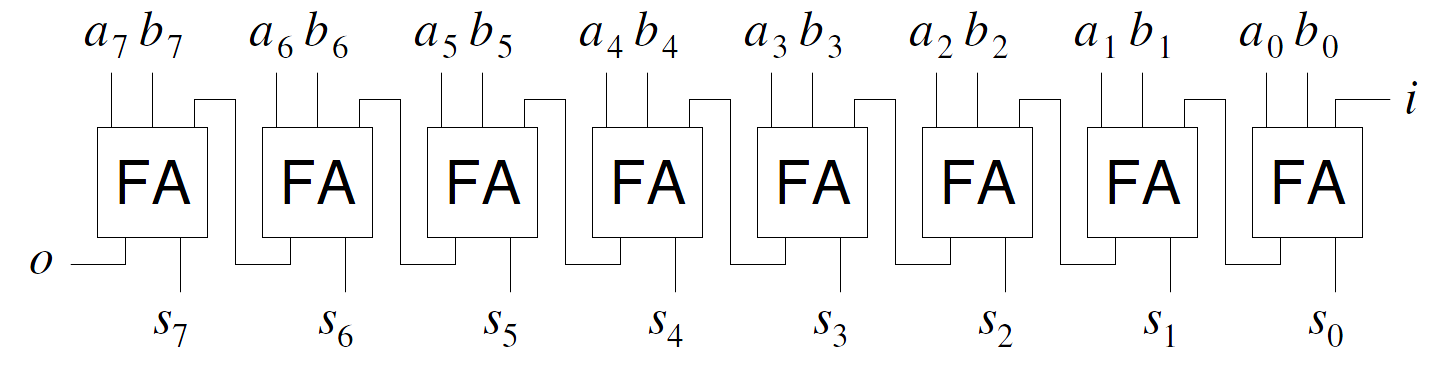
\includegraphics[width = 9cm]{images/arith/ripple.png}
			\end{center}
		
	\end{multicols}
	
	\vspace{8mm}
	
	\subsubsection{Booth Recoding - Multiplikation zweier Binärzahlen ($A \cdot B$)}
	\begin{multicols}{2}
		
			\begin{enumerate}
				\item Wähle kürzere der beiden Zahlen als $A$, wähle $P$ gleich lang wie $B$\\[-5mm]
				\item Erstelle Tabelle $P_{m, \ldots, 0} \mid A_{n, \ldots, 0} \mid A_{-1}$ = 0\\[-5mm]
				\item Wende folgende \emph{Regeln} an, starte bei $i = 0$, Tue bei jedem Schritt: $i := i + 1$:\\[1.5mm]
					\begin{tabular}{l | l | l}
						$A_i$   &   $A_{i-1}$   &   ToDo\\\hline\hline
						0       &   0           &   - \\\hline
						0       &   1           &   addiere B zu P\\\hline
						1       &   0           &   addiere -B zu P\\\hline
						1       &   1           &   -
					\end{tabular}
					\\[-2mm]
				\item Shifte arithmetisch nach rechts (d.h. Vorzeichen nachschieben)\\[-5.5mm]
				\item Wiederhole (3) und (4) $n$ (Länge A) mal\\[-5.5mm]
			\end{enumerate}
			
		\columnbreak
		
			\begin{center}
			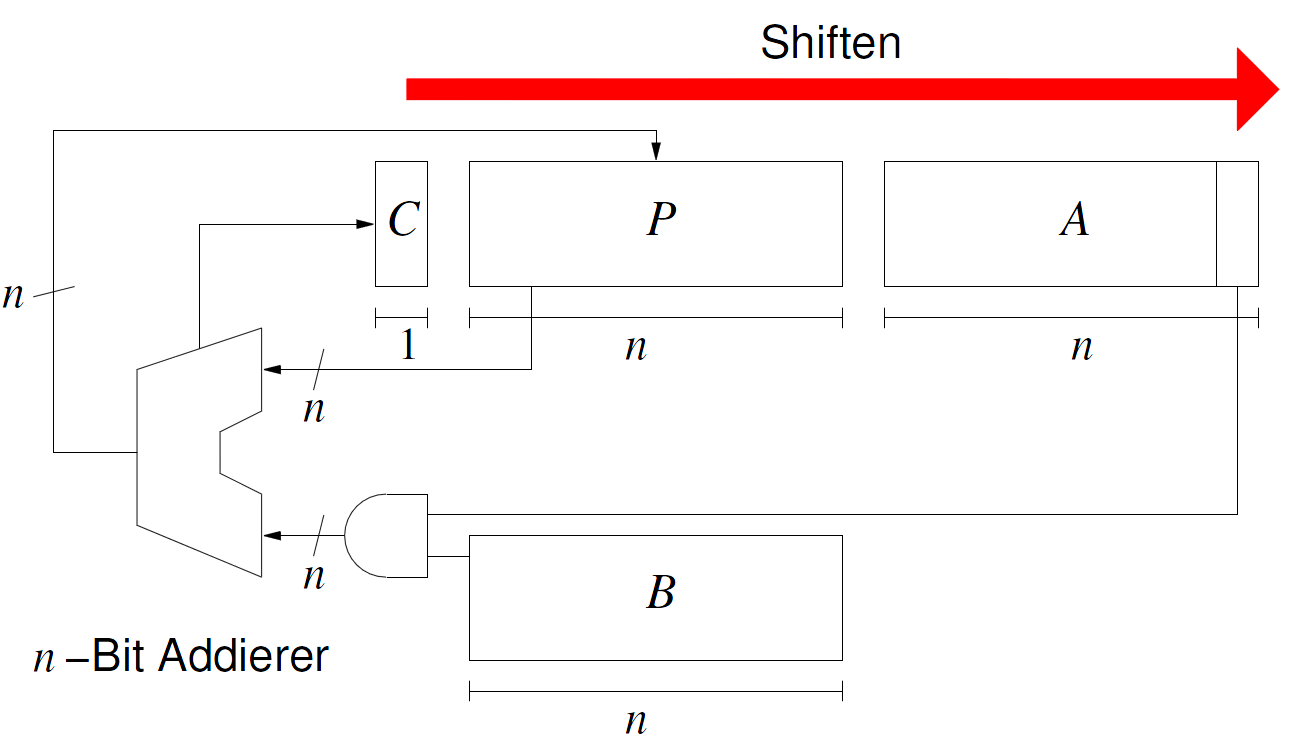
\includegraphics[width = 7cm]{images/arith/mult.png}
			\end{center}
	\end{multicols}

		
		
		
		
		
		
		
		
		
		
		
		
		
		
		
		
		
		
		
		
		
		
		


% die seite füllen
\clearpage


\end{document}


